%------------------------------------------------------------------
% !TEX program = xelatex
% !BIB program = biber
%------------------------------------------------------------------
%&preformat-disser
%\RequirePackage[l2tabu,orthodox]{nag} % Раскомментировав, можно в логе получать рекомендации относительно правильного использования пакетов и предупреждения об устаревших и нерекомендуемых пакетах
% Формат А4, 14pt (ГОСТ Р 7.0.11-2011, 5.3.6)
\documentclass[a4paper,14pt,oneside,openany]{memoir}
%%% Проверка используемого TeX-движка %%%
\RequirePackage{ifxetex, ifluatex}
\newif\ifxetexorluatex   % определяем новый условный оператор (http://tex.stackexchange.com/a/47579)
\ifxetex
    \xetexorluatextrue
\else
    \ifluatex
        \xetexorluatextrue
    \else
        \xetexorluatexfalse
    \fi
\fi

\newif\ifsynopsis           % Условие, проверяющее, что документ --- автореферат
\RequirePackage{etoolbox}[2015/08/02]               % Для продвинутой проверки разных условий

%%% Поля и разметка страницы %%%
\usepackage{pdflscape}                              % Для включения альбомных страниц
\usepackage{geometry}                               % Для последующего задания полей

%%% Математические пакеты %%%
\usepackage{amsthm,amsmath,amscd,amsfonts,amssymb}  % Математические дополнения от AMS
\usepackage{mathtools}                              % Добавляет окружение multlined
\usepackage{unicode-math}
\usepackage{amstext}                               % Русские символы в формулах

%%%% Установки для размера шрифта 14 pt %%%%
%% Формирование переменных и констант для сравнения (один раз для всех подключаемых файлов)%%
%% должно располагаться до вызова пакета fontspec или polyglossia, потому что они сбивают его работу
\newlength{\curtextsize}
\newlength{\bigtextsize}
\setlength{\bigtextsize}{13.9pt}

\makeatletter
%\show\f@size                                       % неплохо для отслеживания, но вызывает стопорение процесса, если документ компилируется без команды  -interaction=nonstopmode
\setlength{\curtextsize}{\f@size pt}
\makeatother

%%% Кодировки и шрифты %%%
\usepackage{polyglossia}[2014/05/21]            % Поддержка многоязычности (fontspec подгружается автоматически)

%%% Оформление абзацев %%%
\usepackage{indentfirst}                            % Красная строка

%%% Цвета %%%
\usepackage[dvipsnames, table, hyperref, cmyk]{xcolor} % Совместимо с tikz. Конвертация всех цветов в cmyk заложена как удовлетворение возможного требования типографий. Возможно конвертирование и в rgb.

%%% Таблицы %%%
\usepackage{longtable,ltcaption}                    % Длинные таблицы
\usepackage{multirow,makecell}                      % Улучшенное форматирование таблиц

%%% Общее форматирование
\usepackage{soulutf8}                               % Поддержка переносоустойчивых подчёркиваний и зачёркиваний
\usepackage{icomma}                                 % Запятая в десятичных дробях
\usepackage[hyphenation, lastparline]{impnattypo}   % Оптимизация расстановки переносов и длины последней строки абзаца

%%% Гиперссылки %%%
\usepackage{hyperref}[2012/11/06]

%%% Изображения %%%
\usepackage{graphicx}[2014/04/25]                   % Подключаем пакет работы с графикой

%%% Списки %%%
\usepackage{enumitem}

%%% Счётчики %%%
\usepackage[figure,table]{totalcount}               % Счётчик рисунков и таблиц
\usepackage{totcount}                               % Пакет создания счётчиков на основе последнего номера подсчитываемого элемента (может требовать дважды компилировать документ)
\usepackage{totpages}                               % Счётчик страниц, совместимый с hyperref (ссылается на номер последней страницы). Желательно ставить последним пакетом в преамбуле
\usepackage{pdfpages}
%%% Продвинутое управление групповыми ссылками (пока только формулами) %%%
\usepackage{cleveref}                           % cleveref корректно считывает язык из настроек polyglossia

\creflabelformat{equation}{#2#1#3}                  % Формат по умолчанию ставил круглые скобки вокруг каждого номера ссылки, теперь просто номера ссылок без какого-либо дополнительного оформления
\crefrangelabelformat{equation}{#3#1#4---#5#2#6}   % Интервалы в русском языке принято делать через тире, если иное не оговорено


%%% Цитата, не приводимая в автореферате:
% возможно, актуальна только для biblatex
%\newcommand{\citeinsynopsis}[1]{\ifsynopsis\else ~\cite{#1} \fi}
            % Пакеты общие для диссертации и автореферата
%%% Прикладные пакеты %%%
%\usepackage{calc}               % Пакет для расчётов параметров, например длины

%%% Для добавления Стр. над номерами страниц в оглавлении
%%% http://tex.stackexchange.com/a/306950
\usepackage{afterpage}

\usepackage{tikz}                   % Продвинутый пакет векторной графики
\usetikzlibrary{chains}             % Для примера tikz рисунка
\usetikzlibrary{shapes.geometric}   % Для примера tikz рисунка
\usetikzlibrary{shapes.symbols}     % Для примера tikz рисунка
\usetikzlibrary{arrows}             % Для примера tikz рисунка

\usepackage[explicit]{titlesec}   %
\usepackage{tocvsec2}               %Подробности оглавления
 \usepackage[normalem]{ulem}
 \useunder{\uline}{\ul}{}
%\usepackage{titlesec}%
%\usepackage{caption}
%\usepackage{subcaption}
%\usepackage{subfig}
         % Пакеты для диссертации
\usepackage{tabu, tabulary}  %таблицы с автоматически подбирающейся шириной столбцов
\usepackage{fr-longtable}    %ради \endlasthead

% Листинги с исходным кодом программ
\usepackage{fancyvrb}
\usepackage{listings}
\lccode`\~=0\relax %Без этого хака из-за особенностей пакета listings перестают работать конструкции с \MakeLowercase и т. п. в (xe|lua)latex

% Русская традиция начертания греческих букв
\usepackage{upgreek} % прямые греческие ради русской традиции

% Микротипографика
%    \usepackage[final]{microtype}[2016/05/14] % улучшает представление букв и слов в строках, может помочь при наличии отдельно висящих слов

        % Пакеты для специфических пользовательских задач

%%%%%%%%%%%%%%%%%%%%%%%%%%%%%%%%%%%%%%%%%%%%%%%%%%%%%%
%%%% Файл упрощённых настроек шаблона диссертации %%%%
%%%%%%%%%%%%%%%%%%%%%%%%%%%%%%%%%%%%%%%%%%%%%%%%%%%%%%

%%% Инициализирование переменных, не трогать!  %%%
\newcounter{intvl}
\newcounter{otstup}
\newcounter{contnumeq}
\newcounter{contnumfig}
\newcounter{contnumtab}
\newcounter{pgnum}
\newcounter{chapstyle}
\newcounter{headingdelim}
\newcounter{headingalign}
\newcounter{headingsize}
\newcounter{tabcap}
\newcounter{tablaba}
\newcounter{tabtita}
\newcounter{usefootcite}
%% Мои указатели
%%%%%%%%%%%%%%%%%%%%%%%%%%%%%%%%%%%%%%%%%%%%%%%%%%

%%% Область упрощённого управления оформлением %%%

%% Интервал между заголовками и между заголовком и текстом
% Заголовки отделяют от текста сверху и снизу тремя интервалами (ГОСТ Р 7.0.11-2011, 5.3.5)
\setcounter{intvl}{2}               % Коэффициент кратности к размеру шрифта

%% Отступы у заголовков в тексте
\setcounter{otstup}{1}              % 0 --- без отступа; 1 --- абзацный отступ

%% Нумерация формул, таблиц и рисунков
\setcounter{contnumeq}{0}           % Нумерация формул: 0 --- пораздельно (во введении подряд, без номера раздела); 1 --- сквозная нумерация по всей диссертации
\setcounter{contnumfig}{0}          % Нумерация рисунков: 0 --- пораздельно (во введении подряд, без номера раздела); 1 --- сквозная нумерация по всей диссертации
\setcounter{contnumtab}{0}          % Нумерация таблиц: 0 --- пораздельно (во введении подряд, без номера раздела); 1 --- сквозная нумерация по всей диссертации

%% Оглавление
\setcounter{pgnum}{0}               % 0 --- номера страниц никак не обозначены; 1 --- Стр. над номерами страниц (дважды компилировать после изменения)
\settocdepth{section}            % до какого уровня подразделов выносить в оглавление
\setsecnumdepth{none}         % до какого уровня нумеровать подразделы


%% Текст и форматирование заголовков
\setcounter{chapstyle}{0}           % 0 --- разделы только под номером; 1 --- разделы с названием "Глава" перед номером
\setcounter{headingdelim}{0}        % 0 --- номер отделен пропуском в 1em или \quad; 1 --- номера разделов и приложений отделены точкой с пробелом, подразделы пропуском без точки; 2 --- номера разделов, подразделов и приложений отделены точкой с пробелом.

%% Выравнивание заголовков в тексте
\setcounter{headingalign}{0}        % 0 --- по центру; 1 --- по левому краю

%% Размеры заголовков в тексте
\setcounter{headingsize}{0}         % 0 --- по ГОСТ, все всегда 14 пт; 1 --- пропорционально изменяющийся размер в зависимости от базового шрифта

%% Подпись таблиц
\setcounter{tabcap}{0}              % 0 --- по ГОСТ, номер таблицы и название разделены тире, выровнены по левому краю, при необходимости на нескольких строках; 1 --- подпись таблицы не по ГОСТ, на двух и более строках, дальнейшие настройки:
%Выравнивание первой строки, с подписью и номером
\setcounter{tablaba}{0}             % 0 --- по левому краю; 1 --- по центру; 2 --- по правому краю
%Выравнивание строк с самим названием таблицы
\setcounter{tabtita}{0}             % 0 --- по левому краю; 1 --- по центру; 2 --- по правому краю
%Разделитель записи «Таблица #» и названия таблицы
\newcommand{\tablabelsep}{\ }

%% Подпись рисунков
%Разделитель записи «Рисунок #» и названия рисунка
\newcommand{\figlabelsep}{~\textemdash\ } % (ГОСТ 2.105, 4.3.1) % "--- здесь не работает

%%% Цвета гиперссылок %%%
% Latex color definitions: http://latexcolor.com/
\definecolor{linkcolor}{rgb}{0.9,0,0}
\definecolor{citecolor}{rgb}{0,0.6,0}
\definecolor{urlcolor}{rgb}{0,0,1}
%\definecolor{linkcolor}{rgb}{0,0,0} %black
%\definecolor{citecolor}{rgb}{0,0,0} %black
%\definecolor{urlcolor}{rgb}{0,0,0} %black
               % Упрощённые настройки шаблона

%%% Переопределение именований, чтобы можно было и в преамбуле использовать %%%
\renewcommand{\chaptername}{Лабораторна робота}
\renewcommand{\appendixname}{Додаток} % (ГОСТ Р 7.0.11-2011, 5.7)
  % Переопределение именований, чтобы можно было и в преамбуле использовать
% Новые переменные, которые могут использоваться во всём проекте
% ГОСТ 7.0.11-2011
% 9.2 Оформление текста автореферата диссертации
% 9.2.1 Общая характеристика работы включает в себя следующие основные структурные
% элементы:
% актуальность темы исследования;
\newcommand{\actualityTXT}{Актуальность темы.}
% степень ее разработанности;
\newcommand{\progressTXT}{Степень разработанности темы.}
% цели и задачи;
\newcommand{\aimTXT}{Целью}
\newcommand{\tasksTXT}{задачи}
% научную новизну;
\newcommand{\noveltyTXT}{Научная новизна:}
% теоретическую и практическую значимость работы;
%\newcommand{\influenceTXT}{Теоретическая и практическая значимость}
% или чаще используют просто
\newcommand{\influenceTXT}{Практическая значимость}
% методологию и методы исследования;
\newcommand{\methodsTXT}{Mетодология и методы исследования.}
% положения, выносимые на защиту;
\newcommand{\defpositionsTXT}{Основные положения, выносимые на~защиту:}
% степень достоверности и апробацию результатов.
\newcommand{\reliabilityTXT}{Достоверность}
\newcommand{\probationTXT}{Апробация работы.}

\newcommand{\contributionTXT}{Личный вклад.}
\newcommand{\publicationsTXT}{Публикации.}


\newcommand{\authorbibtitle}{Публикации автора по теме диссертации}
\newcommand{\vakbibtitle}{В изданиях из списка ВАК РФ}
\newcommand{\notvakbibtitle}{В прочих изданиях}
\newcommand{\confbibtitle}{В сборниках трудов конференций}
\newcommand{\fullbibtitle}{Список використаних джерел}
\newcommand{\conname}{Fernando De Luca}
       % Новые переменные, которые могут использоваться во всём проекте

%%% Основные сведения %%%
\newcommand{\thesisAuthorLastName}{\todo{Фамилия}}
\newcommand{\thesisAuthorOtherNames}{\todo{Имя Отчество}}
\newcommand{\thesisAuthorInitials}{\todo{И.\,О.}}
\newcommand{\thesisAuthor}             % Диссертация, ФИО автора
{%
    \texorpdfstring{% \texorpdfstring takes two arguments and uses the first for (La)TeX and the second for pdf
        \thesisAuthorLastName~\thesisAuthorOtherNames% так будет отображаться на титульном листе или в тексте, где будет использоваться переменная
    }{%
        \thesisAuthorLastName, \thesisAuthorOtherNames% эта запись для свойств pdf-файла. В таком виде, если pdf будет обработан программами для сбора библиографических сведений, будет правильно представлена фамилия.
    }
}
\newcommand{\thesisAuthorShort}        % Диссертация, ФИО автора инициалами
{\thesisAuthorInitials~\thesisAuthorLastName}
%\newcommand{\thesisUdk}                % Диссертация, УДК
%{\todo{xxx.xxx}}
\newcommand{\thesisTitle}              % Диссертация, название
{\todo{Название диссертационной работы}}
\newcommand{\thesisSpecialtyNumber}    % Диссертация, специальность, номер
{\todo{XX.XX.XX}}
\newcommand{\thesisSpecialtyTitle}     % Диссертация, специальность, название
{\todo{Название специальности}}
\newcommand{\thesisDegree}             % Диссертация, ученая степень
{\todo{кандидата физико-математических наук}}
\newcommand{\thesisDegreeShort}        % Диссертация, ученая степень, краткая запись
{\todo{канд. физ.-мат. наук}}
\newcommand{\thesisCity}               % Диссертация, город написания диссертации
{\todo{Город}}
\newcommand{\thesisYear}               % Диссертация, год написания диссертации
{\todo{20XX}}
\newcommand{\thesisOrganization}       % Диссертация, организация
{\todo{Название учреждения, в~котором выполнялась данная диссертационная работа}}
\newcommand{\thesisOrganizationShort}  % Диссертация, краткое название организации для доклада
{\todo{НазУчДисРаб}}

\newcommand{\thesisInOrganization}     % Диссертация, организация в предложном падеже: Работа выполнена в ...
{\todo{учреждении, в~котором выполнялась данная диссертационная работа}}

\newcommand{\supervisorFio}            % Научный руководитель, ФИО
{\todo{Фамилия Имя Отчество}}
\newcommand{\supervisorRegalia}        % Научный руководитель, регалии
{\todo{уч. степень, уч. звание}}
\newcommand{\supervisorFioShort}       % Научный руководитель, ФИО
{\todo{И.\,О.~Фамилия}}
\newcommand{\supervisorRegaliaShort}   % Научный руководитель, регалии
{\todo{уч.~ст.,~уч.~зв.}}


\newcommand{\opponentOneFio}           % Оппонент 1, ФИО
{\todo{Фамилия Имя Отчество}}
\newcommand{\opponentOneRegalia}       % Оппонент 1, регалии
{\todo{доктор физико-математических наук, профессор}}
\newcommand{\opponentOneJobPlace}      % Оппонент 1, место работы
{\todo{Не очень длинное название для места работы}}
\newcommand{\opponentOneJobPost}       % Оппонент 1, должность
{\todo{старший научный сотрудник}}

\newcommand{\opponentTwoFio}           % Оппонент 2, ФИО
{\todo{Фамилия Имя Отчество}}
\newcommand{\opponentTwoRegalia}       % Оппонент 2, регалии
{\todo{кандидат физико-математических наук}}
\newcommand{\opponentTwoJobPlace}      % Оппонент 2, место работы
{\todo{Основное место работы c длинным длинным длинным длинным названием}}
\newcommand{\opponentTwoJobPost}       % Оппонент 2, должность
{\todo{старший научный сотрудник}}

\newcommand{\leadingOrganizationTitle} % Ведущая организация, дополнительные строки
{\todo{Федеральное государственное бюджетное образовательное учреждение высшего профессионального образования с~длинным длинным длинным длинным названием}}

\newcommand{\defenseDate}              % Защита, дата
{\todo{DD mmmmmmmm YYYY~г.~в~XX часов}}
\newcommand{\defenseCouncilNumber}     % Защита, номер диссертационного совета
{\todo{Д\,123.456.78}}
\newcommand{\defenseCouncilTitle}      % Защита, учреждение диссертационного совета
{\todo{Название учреждения}}
\newcommand{\defenseCouncilAddress}    % Защита, адрес учреждение диссертационного совета
{\todo{Адрес}}
\newcommand{\defenseCouncilPhone}      % Телефон для справок
{\todo{+7~(0000)~00-00-00}}

\newcommand{\defenseSecretaryFio}      % Секретарь диссертационного совета, ФИО
{\todo{Фамилия Имя Отчество}}
\newcommand{\defenseSecretaryRegalia}  % Секретарь диссертационного совета, регалии
{\todo{д-р~физ.-мат. наук}}            % Для сокращений есть ГОСТы, например: ГОСТ Р 7.0.12-2011 + http://base.garant.ru/179724/#block_30000

\newcommand{\synopsisLibrary}          % Автореферат, название библиотеки
{\todo{Название библиотеки}}
\newcommand{\synopsisDate}             % Автореферат, дата рассылки
{\todo{DD mmmmmmmm YYYY года}}

% To avoid conflict with beamer class use \providecommand
\providecommand{\keywords}%            % Ключевые слова для метаданных PDF диссертации и автореферата
{}
           % Основные сведения
%%% Шаблон %%%
\DeclareRobustCommand{\todo}{\textcolor{red}}       % решаем проблему превращения названия цвета в результате \MakeUppercase, http://tex.stackexchange.com/a/187930/79756 , \DeclareRobustCommand protects \todo from expanding inside \MakeUppercase
\AtBeginDocument{%
    \setlength{\parindent}{2.5em}                   % Абзацный отступ. Должен быть одинаковым по всему тексту и равен пяти знакам (ГОСТ Р 7.0.11-2011, 5.3.7).
}

%%% Кодировки и шрифты %%%
\setmainlanguage{ukrainian}  % Язык по-умолчанию русский с поддержкой приятных команд пакета babel
\setotherlanguages{russian,english}                       % Дополнительный язык = английский (в американской вариации по-умолчанию)
\setmonofont{Courier New}                        % моноширинный шрифт
\newfontfamily\cyrillicfonttt{Courier New}       % моноширинный шрифт для кириллицы
\defaultfontfeatures{Ligatures=TeX}              % стандартные лигатуры TeX, замены нескольких дефисов на тире и т. п. Настройки моноширинного шрифта должны идти до этой строки, чтобы при врезках кода программ в коде не применялись лигатуры и замены дефисов
\setmainfont{Times New Roman}                    % Шрифт с засечками
\newfontfamily\cyrillicfont{Times New Roman}     % Шрифт с засечками для кириллицы
\setsansfont{Arial}                              % Шрифт без засечек
\newfontfamily\cyrillicfontsf{Arial}             % Шрифт без засечек для кириллицы


%%% Подписи %%%
\setlength{\abovecaptionskip}{0pt}   % Отбивка над подписью
\setlength{\belowcaptionskip}{0pt}   % Отбивка под подписью
\captionwidth{\linewidth}
\normalcaptionwidth

%%% Таблицы %%%
\ifnumequal{\value{tabcap}}{0}{%
    \newcommand{\tabcapalign}{\raggedright \hspace{2.5em}}  % по левому краю страницы или аналога parbox
    \renewcommand{\tablabelsep}{~\textemdash\ } % тире как разделитель идентификатора с номером от наименования
    \newcommand{\tabtitalign}{}
}{%
    \ifnumequal{\value{tablaba}}{0}{%
        \newcommand{\tabcapalign}{\raggedright}  % по левому краю страницы или аналога parbox
    }{}

    \ifnumequal{\value{tablaba}}{1}{%
        \newcommand{\tabcapalign}{\centering}    % по центру страницы или аналога parbox
    }{}

    \ifnumequal{\value{tablaba}}{2}{%
        \newcommand{\tabcapalign}{\raggedleft}   % по правому краю страницы или аналога parbox
    }{}

    \ifnumequal{\value{tabtita}}{0}{%
        \newcommand{\tabtitalign}{\par\raggedright}  % по левому краю страницы или аналога parbox
    }{}

    \ifnumequal{\value{tabtita}}{1}{%
        \newcommand{\tabtitalign}{\par\centering}    % по центру страницы или аналога parbox
    }{}

    \ifnumequal{\value{tabtita}}{2}{%
        \newcommand{\tabtitalign}{\par\raggedleft}   % по правому краю страницы или аналога parbox
    }{}
}

\precaption{\tabcapalign} % всегда идет перед подписью или \legend
\captionnamefont{\normalfont\normalsize} % Шрифт надписи «Таблица #»; также определяет шрифт у \legend
\captiondelim{\tablabelsep} % разделитель идентификатора с номером от наименования
\captionstyle[\tabtitalign]{\tabtitalign}
\captiontitlefont{\normalfont\normalsize} % Шрифт с текстом подписи


%%% Рисунки %%%
\setfloatadjustment{figure}{%
    \setlength{\abovecaptionskip}{0pt}   % Отбивка над подписью
    \setlength{\belowcaptionskip}{0pt}   % Отбивка под подписью
    \precaption{} % всегда идет перед подписью или \legend
    \captionnamefont{\normalfont\normalsize} % Шрифт надписи «Рисунок #»; также определяет шрифт у \legend
    \captiondelim{\figlabelsep} % разделитель идентификатора с номером от наименования
    \captionstyle[\centering]{\centering} % Центрирование подписей, заданных командой \caption и \legend
    \captiontitlefont{\normalfont\normalsize} % Шрифт с текстом подписи
    \postcaption{} % всегда идет после подписи или \legend, и с новой строки
}

%%% Подписи подрисунков %%%
\newsubfloat{figure} % Включает возможность использовать подрисунки у окружений figure
\renewcommand{\thesubfigure}{\asbuk{subfigure}}           % Буквенные номера подрисунков
\subcaptionsize{\normalsize} % Шрифт подписи названий подрисунков (не отличается от основного)
\subcaptionlabelfont{\normalfont}
\subcaptionfont{\!\!) \normalfont} % Вот так тут добавили скобку после буквы.
\subcaptionstyle{\centering}
%\subcaptionsize{\fontsize{12pt}{13pt}\selectfont} % объявляем шрифт 12pt для использования в подписях, тут же надо интерлиньяж объявлять, если не наследуется

%%% Настройки гиперссылок %%%
\ifluatex
    \hypersetup{
        unicode,                % Unicode encoded PDF strings
    }
\fi

\hypersetup{
    linktocpage=true,           % ссылки с номера страницы в оглавлении, списке таблиц и списке рисунков
%    linktoc=all,                % both the section and page part are links
%    pdfpagelabels=false,        % set PDF page labels (true|false)
    plainpages=false,           % Forces page anchors to be named by the Arabic form  of the page number, rather than the formatted form
    colorlinks,                 % ссылки отображаются раскрашенным текстом, а не раскрашенным прямоугольником, вокруг текста
    linkcolor={linkcolor},      % цвет ссылок типа ref, eqref и подобных
    citecolor={citecolor},      % цвет ссылок-цитат
    urlcolor={urlcolor},        % цвет гиперссылок
%    hidelinks,                  % Hide links (removing color and border)
    pdftitle={\thesisTitle},    % Заголовок
    pdfauthor={\thesisAuthor},  % Автор
    pdfsubject={\thesisSpecialtyNumber\ \thesisSpecialtyTitle},      % Тема
%    pdfcreator={Создатель},     % Создатель, Приложение
%    pdfproducer={Производитель},% Производитель, Производитель PDF
    pdfkeywords={\keywords},    % Ключевые слова
    pdflang={ru},
}

%%% Списки %%%
% Используем короткое тире (endash) для ненумерованных списков (ГОСТ 2.105-95, пункт 4.1.7, требует дефиса, но так лучше смотрится)
\renewcommand{\labelitemi}{\normalfont\bfseries{--}}

% Перечисление строчными буквами латинского алфавита (ГОСТ 2.105-95, 4.1.7)
%\renewcommand{\theenumi}{\alph{enumi}}
%\renewcommand{\labelenumi}{\theenumi)}

% Перечисление строчными буквами русского алфавита (ГОСТ 2.105-95, 4.1.7)
\makeatletter
\AddEnumerateCounter{\asbuk}{\russian@alph}{щ}      % Управляем списками/перечислениями через пакет enumitem, а он 'не знает' про asbuk, потому 'учим' его
\makeatother
%\renewcommand{\theenumi}{\asbuk{enumi}} %первый уровень нумерации
%\renewcommand{\labelenumi}{\theenumi)} %первый уровень нумерации
\renewcommand{\theenumii}{\asbuk{enumii}} %второй уровень нумерации
\renewcommand{\labelenumii}{\theenumii)} %второй уровень нумерации
\renewcommand{\theenumiii}{\arabic{enumiii}} %третий уровень нумерации
\renewcommand{\labelenumiii}{\theenumiii)} %третий уровень нумерации

\setlist{nosep,%                                    % Единый стиль для всех списков (пакет enumitem), без дополнительных интервалов.
    labelindent=\parindent,leftmargin=*%            % Каждый пункт, подпункт и перечисление записывают с абзацного отступа (ГОСТ 2.105-95, 4.1.8)
}
              % Стили общие для диссертации и автореферата

%%% Изображения %%%
\graphicspath{{images/}}         % Пути к изображениям

%%% Макет страницы %%%
% Выставляем значения полей (ГОСТ 7.0.11-2011, 5.3.7)
\geometry{a4paper,top=2cm,bottom=2cm,left=2.5cm,right=1cm,nofoot,nomarginpar} %,showframe
\setlength{\topskip}{0pt}   %размер дополнительного верхнего поля
\setlength{\footskip}{12.3pt} % снимет warning, согласно https://tex.stackexchange.com/a/334346

%%% Интервалы %%%
%% По ГОСТ Р 7.0.11-2011, пункту 5.3.6 требуется полуторный интервал
%% Реализация средствами класса (на основе setspace) ближе к типографской классике.
%% И правит сразу и в таблицах (если со звёздочкой)
%\DoubleSpacing*     % Двойной интервал
\OnehalfSpacing*    % Полуторный интервал
%\setSpacing{1.42}   % Полуторный интервал, подобный Ворду (возможно, стоит включать вместе с предыдущей строкой)

%%% Выравнивание и переносы %%%
%% http://tex.stackexchange.com/questions/241343/what-is-the-meaning-of-fussy-sloppy-emergencystretch-tolerance-hbadness
%% http://www.latex-community.org/forum/viewtopic.php?p=70342#p70342
\tolerance 1414 %
\hbadness 1414%
\emergencystretch 1.5em % В случае проблем регулировать в первую очередь
\hfuzz 0.3pt
\vfuzz \hfuzz
%\raggedbottom
\sloppy                 % Избавляемся от переполнений
\clubpenalty=10000      % Запрещаем разрыв страницы после первой строки абзаца
\flushbottom
\widowpenalty=4991     % Запрещаем разрыв страницы после последней строки абзаца


%%% Блок управления параметрами для выравнивания заголовков в тексте %%%
\newlength{\otstuplen}
\setlength{\otstuplen}{\theotstup\parindent}
\ifnumequal{\value{headingalign}}{0}{% выравнивание заголовков в тексте
    \newcommand{\hdngalign}{\centering}                % по центру
    \newcommand{\hdngaligni}{}% по центру
    \setlength{\otstuplen}{0pt}
}{%
    \newcommand{\hdngalign}{}                 % по левому краю
    \newcommand{\hdngaligni}{\hspace{\otstuplen}}      % по левому краю
} % В обоих случаях вроде бы без переноса, как и надо (ГОСТ Р 7.0.11-2011, 5.3.5)

%%% Оглавление %%%
\renewcommand{\cftchapterdotsep}{\cftdotsep}                % отбивка точками до номера страницы начала главы/раздела

%% Переносить слова в заголовке не допускается (ГОСТ Р 7.0.11-2011, 5.3.5). Заголовки в оглавлении должны точно повторять заголовки в тексте (ГОСТ Р 7.0.11-2011, 5.2.3). Прямого указания на запрет переносов в оглавлении нет, но по той же логике невнесения искажений в смысл, лучше в оглавлении не переносить:
\setrmarg{2.55em plus1fil}                             %To have the (sectional) titles in the ToC, etc., typeset ragged right with no hyphenation
\renewcommand{\cftchapterpagefont}{\normalfont}        % нежирные номера страниц у глав в оглавлении
\renewcommand{\cftchapterleader}{\cftdotfill{\cftchapterdotsep}}% нежирные точки до номеров страниц у глав в оглавлении
%\renewcommand{\cftchapterfont}{}                       % нежирные названия глав в оглавлении

\ifnumgreater{\value{headingdelim}}{0}{%
    \renewcommand\cftchapteraftersnum{.\space}       % добавляет точку с пробелом после номера раздела в оглавлении
}{}
\ifnumgreater{\value{headingdelim}}{1}{%
    \renewcommand\cftsectionaftersnum{.\space}       % добавляет точку с пробелом после номера подраздела в оглавлении
    \renewcommand\cftsubsectionaftersnum{.\space}    % добавляет точку с пробелом после номера подподраздела в оглавлении
    \renewcommand\cftsubsubsectionaftersnum{.\space} % добавляет точку с пробелом после номера подподподраздела в оглавлении
    \AtBeginDocument{% без этого polyglossia сама всё переопределяет
        \setsecnumformat{\csname the#1\endcsname.\space}
    }
}{%
    \AtBeginDocument{% без этого polyglossia сама всё переопределяет
        \setsecnumformat{\csname the#1\endcsname\quad}
    }
}
\renewcommand*{\cftappendixname}{\appendixname\space} % Слово Приложение в оглавлении

%%% Колонтитулы %%%
% Порядковый номер страницы печатают на середине верхнего поля страницы (ГОСТ Р 7.0.11-2011, 5.3.8)
\makeevenhead{plain}{}{}{\thepage}%
 \makeoddhead{plain}{}{}{\thepage}%
\makeevenfoot{plain}{}{}{}%
\makeoddfoot{plain}{}{}{}%
\pagestyle{plain}%

%%% добавить Стр. над номерами страниц в оглавлении
%%% http://tex.stackexchange.com/a/306950
\newif\ifendTOC

\newcommand*{\tocheader}{
\ifnumequal{\value{pgnum}}{1}{%
    \ifendTOC\else\hbox to \linewidth%
      {\noindent{}~\hfill{Стр.}}\par%
      \ifnumless{\value{page}}{3}{}{%
        \vspace{0.5\onelineskip}
      }
      \afterpage{\tocheader}
    \fi%
}{}%
}%

%%% Оформление заголовков глав, разделов, подразделов %%%
%% Работа должна быть выполнена ... размером шрифта 12-14 пунктов (ГОСТ Р 7.0.11-2011, 5.3.8). То есть не должно быть надписей шрифтом более 14. Так и поставим.
%% Эти установки будут давать одинаковый результат независимо от выбора базовым шрифтом 12 пт или 14 пт
\newcommand{\basegostsectionfont}{\fontsize{14pt}{16pt}\selectfont\bfseries}

\makechapterstyle{thesisgost}{%
    \chapterstyle{default}
    \setlength{\beforechapskip}{0pt}
    \setlength{\midchapskip}{0pt}
    \setlength{\afterchapskip}{\theintvl\curtextsize}
    \renewcommand*{\chapnamefont}{\basegostsectionfont}
    \renewcommand*{\chapnumfont}{\basegostsectionfont}
    \renewcommand*{\chaptitlefont}{\basegostsectionfont}
    \renewcommand*{\chapterheadstart}{}
    \ifnumgreater{\value{headingdelim}}{0}{%
        \renewcommand*{\afterchapternum}{.\space}   % добавляет точку с пробелом после номера раздела
    }{%
        \renewcommand*{\afterchapternum}{\quad}     % добавляет \quad после номера раздела
    }
    \renewcommand*{\printchapternum}{\hdngaligni\hdngalign\chapnumfont \thechapter}
    \renewcommand*{\printchaptername}{}
    \renewcommand*{\printchapternonum}{\hdngaligni\hdngalign}
}

\makeatletter
\makechapterstyle{thesisgostchapname}{%
    \chapterstyle{thesisgost}
    \renewcommand*{\printchapternum}{\chapnumfont \thechapter}
    \renewcommand*{\printchaptername}{\hdngaligni\hdngalign\chapnamefont \@makechapterhead} %
}
\makeatother

\chapterstyle{thesisgost}

\setsecheadstyle{\basegostsectionfont\hdngalign}
\setsecindent{\otstuplen}

\setsubsecheadstyle{\basegostsectionfont\hdngalign}
\setsubsecindent{\otstuplen}

\setsubsubsecheadstyle{\basegostsectionfont\hdngalign}
\setsubsubsecindent{\otstuplen}

\sethangfrom{\noindent #1} %все заголовки подразделов центрируются с учетом номера, как block

\ifnumequal{\value{chapstyle}}{1}{%
    \chapterstyle{thesisgostchapname}
    \renewcommand*{\cftchaptername}{\chaptertitlename\space} % будет вписано слово Глава перед каждым номером раздела в оглавлении
}{}%


%%% Интервалы между заголовками
%\setbeforesecskip{\theintvl\curtextsize}% Заголовки отделяют от текста сверху и снизу тремя интервалами (ГОСТ Р 7.0.11-2011, 5.3.5).
%\setaftersecskip{\theintvl\curtextsize}
%\setbeforesubsecskip{\theintvl\curtextsize}
%\setaftersubsecskip{\theintvl\curtextsize}
%\setbeforesubsubsecskip{\theintvl\curtextsize}
%\setaftersubsubsecskip{\theintvl\curtextsize}

\setbeforesecskip{0.8ex} \setaftersecskip{0.7ex} \setbeforesubsecskip{0.8ex}
\setaftersubsecskip{0.7ex} \setbeforesubsubsecskip{0.8ex}
\setaftersubsubsecskip{0.7ex}

%%% Блок дополнительного управления размерами заголовков
\ifnumequal{\value{headingsize}}{1}{% Пропорциональные заголовки и базовый шрифт 14 пт
    \renewcommand{\basegostsectionfont}{\large\bfseries}
    \renewcommand*{\chapnamefont}{\Large\bfseries}
    \renewcommand*{\chapnumfont}{\Large\bfseries}
    \renewcommand*{\chaptitlefont}{\Large\bfseries}
}{}

%%% Счётчики %%%

%% Упрощённые настройки шаблона диссертации: нумерация формул, таблиц, рисунков
\ifnumequal{\value{contnumeq}}{1}{%
    \counterwithout{equation}{chapter} % Убираем связанность номера формулы с номером главы/раздела
}{}
\ifnumequal{\value{contnumfig}}{1}{%
    \counterwithout{figure}{chapter}   % Убираем связанность номера рисунка с номером главы/раздела
}{}
\ifnumequal{\value{contnumtab}}{1}{%
    \counterwithout{table}{chapter}    % Убираем связанность номера таблицы с номером главы/раздела
}{}


%%http://www.linux.org.ru/forum/general/6993203#comment-6994589 (используется totcount)
\makeatletter
\def\formbytotal#1#2#3#4#5{%
    \newcount\@c
    \@c\totvalue{#1}\relax
    \newcount\@last
    \newcount\@pnul
    \@last\@c\relax
    \divide\@last 10
    \@pnul\@last\relax
    \divide\@pnul 10
    \multiply\@pnul-10
    \advance\@pnul\@last
    \multiply\@last-10
    \advance\@last\@c
    \total{#1}~#2%
    \ifnum\@pnul=1#5\else%
    \ifcase\@last#5\or#3\or#4\or#4\or#4\else#5\fi
    \fi
}
\makeatother

\AtBeginDocument{
%% регистрируем счётчики в системе totcounter
    \regtotcounter{totalcount@figure}
    \regtotcounter{totalcount@table}       % Если иным способом поставить в преамбуле то ошибка в числе таблиц
    \regtotcounter{TotPages}               % Если иным способом поставить в преамбуле то ошибка в числе страниц
}

%%% Правильная нумерация приложений %%%
%% По ГОСТ 2.105, п. 4.3.8 Приложения обозначают заглавными буквами русского алфавита,
%% начиная с А, за исключением букв Ё, З, Й, О, Ч, Ь, Ы, Ъ.
%% Здесь также переделаны все нумерации русскими буквами.

\makeatletter
\def\russian@Alph#1{\ifcase#1\or
    А\or Б\or В\or Г\or Д\or Е\or Ж\or
    И\or К\or Л\or М\or Н\or
    П\or Р\or С\or Т\or У\or Ф\or Х\or
    Ц\or Ш\or Щ\or Э\or Ю\or Я\else\xpg@ill@value{#1}{russian@Alph}\fi}
\def\russian@alph#1{\ifcase#1\or
   а\or б\or в\or г\or д\or е\or ж\or
   и\or к\or л\or м\or н\or
   п\or р\or с\or т\or у\or ф\or х\or
   ц\or ш\or щ\or э\or ю\or я\else\xpg@ill@value{#1}{russian@alph}\fi}
\makeatother
           % Стили для диссертации
% для вертикального центрирования ячеек в tabulary
\def\zz{\ifx\[$\else\aftergroup\zzz\fi}
%$ \] % <-- чиним подсветку синтаксиса в некоторых редакторах
\def\zzz{\setbox0\lastbox
\dimen0\dimexpr\extrarowheight + \ht0-\dp0\relax
\setbox0\hbox{\raise-.5\dimen0\box0}%
\ht0=\dimexpr\ht0+\extrarowheight\relax
\dp0=\dimexpr\dp0+\extrarowheight\relax
\box0
}



\lstdefinelanguage{Renhanced}%
{keywords={abbreviate,abline,abs,acos,acosh,action,add1,add,%
        aggregate,alias,Alias,alist,all,anova,any,aov,aperm,append,apply,%
        approx,approxfun,apropos,Arg,args,array,arrows,as,asin,asinh,%
        atan,atan2,atanh,attach,attr,attributes,autoload,autoloader,ave,%
        axis,backsolve,barplot,basename,besselI,besselJ,besselK,besselY,%
        beta,binomial,body,box,boxplot,break,browser,bug,builtins,bxp,by,%
        c,C,call,Call,case,cat,category,cbind,ceiling,character,char,%
        charmatch,check,chol,chol2inv,choose,chull,class,close,cm,codes,%
        coef,coefficients,co,col,colnames,colors,colours,commandArgs,%
        comment,complete,complex,conflicts,Conj,contents,contour,%
        contrasts,contr,control,helmert,contrib,convolve,cooks,coords,%
        distance,coplot,cor,cos,cosh,count,fields,cov,covratio,wt,CRAN,%
        create,crossprod,cummax,cummin,cumprod,cumsum,curve,cut,cycle,D,%
        data,dataentry,date,dbeta,dbinom,dcauchy,dchisq,de,debug,%
        debugger,Defunct,default,delay,delete,deltat,demo,de,density,%
        deparse,dependencies,Deprecated,deriv,description,detach,%
        dev2bitmap,dev,cur,deviance,off,prev,,dexp,df,dfbetas,dffits,%
        dgamma,dgeom,dget,dhyper,diag,diff,digamma,dim,dimnames,dir,%
        dirname,dlnorm,dlogis,dnbinom,dnchisq,dnorm,do,dotplot,double,%
        download,dpois,dput,drop,drop1,dsignrank,dt,dummy,dump,dunif,%
        duplicated,dweibull,dwilcox,dyn,edit,eff,effects,eigen,else,%
        emacs,end,environment,env,erase,eval,equal,evalq,example,exists,%
        exit,exp,expand,expression,External,extract,extractAIC,factor,%
        fail,family,fft,file,filled,find,fitted,fivenum,fix,floor,for,%
        For,formals,format,formatC,formula,Fortran,forwardsolve,frame,%
        frequency,ftable,ftable2table,function,gamma,Gamma,gammaCody,%
        gaussian,gc,gcinfo,gctorture,get,getenv,geterrmessage,getOption,%
        getwd,gl,glm,globalenv,gnome,GNOME,graphics,gray,grep,grey,grid,%
        gsub,hasTsp,hat,heat,help,hist,home,hsv,httpclient,I,identify,if,%
        ifelse,Im,image,\%in\%,index,influence,measures,inherits,install,%
        installed,integer,interaction,interactive,Internal,intersect,%
        inverse,invisible,IQR,is,jitter,kappa,kronecker,labels,lapply,%
        layout,lbeta,lchoose,lcm,legend,length,levels,lgamma,library,%
        licence,license,lines,list,lm,load,local,locator,log,log10,log1p,%
        log2,logical,loglin,lower,lowess,ls,lsfit,lsf,ls,machine,Machine,%
        mad,mahalanobis,make,link,margin,match,Math,matlines,mat,matplot,%
        matpoints,matrix,max,mean,median,memory,menu,merge,methods,min,%
        missing,Mod,mode,model,response,mosaicplot,mtext,mvfft,na,nan,%
        names,omit,nargs,nchar,ncol,NCOL,new,next,NextMethod,nextn,%
        nlevels,nlm,noquote,NotYetImplemented,NotYetUsed,nrow,NROW,null,%
        numeric,\%o\%,objects,offset,old,on,Ops,optim,optimise,optimize,%
        options,or,order,ordered,outer,package,packages,page,pairlist,%
        pairs,palette,panel,par,parent,parse,paste,path,pbeta,pbinom,%
        pcauchy,pchisq,pentagamma,persp,pexp,pf,pgamma,pgeom,phyper,pico,%
        pictex,piechart,Platform,plnorm,plogis,plot,pmatch,pmax,pmin,%
        pnbinom,pnchisq,pnorm,points,poisson,poly,polygon,polyroot,pos,%
        postscript,power,ppoints,ppois,predict,preplot,pretty,Primitive,%
        print,prmatrix,proc,prod,profile,proj,prompt,prop,provide,%
        psignrank,ps,pt,ptukey,punif,pweibull,pwilcox,q,qbeta,qbinom,%
        qcauchy,qchisq,qexp,qf,qgamma,qgeom,qhyper,qlnorm,qlogis,qnbinom,%
        qnchisq,qnorm,qpois,qqline,qqnorm,qqplot,qr,Q,qty,qy,qsignrank,%
        qt,qtukey,quantile,quasi,quit,qunif,quote,qweibull,qwilcox,%
        rainbow,range,rank,rbeta,rbind,rbinom,rcauchy,rchisq,Re,read,csv,%
        csv2,fwf,readline,socket,real,Recall,rect,reformulate,regexpr,%
        relevel,remove,rep,repeat,replace,replications,report,require,%
        resid,residuals,restart,return,rev,rexp,rf,rgamma,rgb,rgeom,R,%
        rhyper,rle,rlnorm,rlogis,rm,rnbinom,RNGkind,rnorm,round,row,%
        rownames,rowsum,rpois,rsignrank,rstandard,rstudent,rt,rug,runif,%
        rweibull,rwilcox,sample,sapply,save,scale,scan,scan,screen,sd,se,%
        search,searchpaths,segments,seq,sequence,setdiff,setequal,set,%
        setwd,show,sign,signif,sin,single,sinh,sink,solve,sort,source,%
        spline,splinefun,split,sqrt,stars,start,stat,stem,step,stop,%
        storage,strstrheight,stripplot,strsplit,structure,strwidth,sub,%
        subset,substitute,substr,substring,sum,summary,sunflowerplot,svd,%
        sweep,switch,symbol,symbols,symnum,sys,status,system,t,table,%
        tabulate,tan,tanh,tapply,tempfile,terms,terrain,tetragamma,text,%
        time,title,topo,trace,traceback,transform,tri,trigamma,trunc,try,%
        ts,tsp,typeof,unclass,undebug,undoc,union,unique,uniroot,unix,%
        unlink,unlist,unname,untrace,update,upper,url,UseMethod,var,%
        variable,vector,Version,vi,warning,warnings,weighted,weights,%
        which,while,window,write,\%x\%,x11,X11,xedit,xemacs,xinch,xor,%
        xpdrows,xy,xyinch,yinch,zapsmall,zip},%
    otherkeywords={!,!=,~,$,*,\%,\&,\%/\%,\%*\%,\%\%,<-,<<-},%$
    alsoother={._$},%$
    sensitive,%
    morecomment=[l]\#,%
    morestring=[d]",%
    morestring=[d]'% 2001 Robert Denham
}%

% Ширина текста минус ширина надписи 999
\newlength{\twless}
\newlength{\lmarg}
\setlength{\lmarg}{\widthof{999}}   % ширина надписи 999
\setlength{\twless}{\textwidth-\lmarg}


\lstset{ %
%    language=R,                    %  Язык указать здесь, если во всех листингах преимущественно один язык, в результате часть настроек может пойти только для этого языка
    numbers=left,                   % where to put the line-numbers
    numberstyle=\fontsize{12pt}{14pt}\selectfont\color{Gray},  % the style that is used for the line-numbers
    firstnumber=1,                  % в этой и следующей строках задаётся поведение нумерации 5, 10, 15...
    stepnumber=5,                   % the step between two line-numbers. If it's 1, each line will be numbered
    numbersep=5pt,                  % how far the line-numbers are from the code
    backgroundcolor=\color{white},  % choose the background color. You must add \usepackage{color}
    showspaces=false,               % show spaces adding particular underscores
    showstringspaces=false,         % underline spaces within strings
    showtabs=false,                 % show tabs within strings adding particular underscores
    frame=leftline,                 % adds a frame of different types around the code
    rulecolor=\color{black},        % if not set, the frame-color may be changed on line-breaks within not-black text (e.g. commens (green here))
    tabsize=2,                      % sets default tabsize to 2 spaces
    captionpos=t,                   % sets the caption-position to top
    breaklines=true,                % sets automatic line breaking
    breakatwhitespace=false,        % sets if automatic breaks should only happen at whitespace
%    title=\lstname,                 % show the filename of files included with \lstinputlisting;
    % also try caption instead of title
    basicstyle=\fontsize{10pt}{12pt}\selectfont\ttfamily,% the size of the fonts that are used for the code
%    keywordstyle=\color{blue},      % keyword style
    commentstyle=\color{ForestGreen}\emph,% comment style
    stringstyle=\color{Mahogany},   % string literal style
    escapeinside={\%*}{*)},         % if you want to add a comment within your code
    morekeywords={*,...},           % if you want to add more keywords to the set
    xleftmargin={\lmarg},           % Чтобы весь код и полоска с номерами строк была смещена влево, так чтобы цифры не вылезали за пределы текста слева
    inputencoding=utf8,             % кодировка кода
    %extendedchars={false},
    %keepspaces={true}
} %\captiondelim{~\textemdash\ }     % Разделитель для листингов
\lstset{ %
    inputencoding=utf8x,             % кириллица в листингах
    extendedchars={false},          % для XeLaTeX и LuaTeX
    keepspaces={true}               %
    }

%http://tex.stackexchange.com/questions/26872/smaller-frame-with-listings
% Окружение, чтобы листинг был компактнее обведен рамкой, если она задается, а не на всю ширину текста
\makeatletter
\newenvironment{SmallListing}[1][]
{\lstset{#1}\VerbatimEnvironment\begin{VerbatimOut}{VerbEnv.tmp}}
{\end{VerbatimOut}\settowidth\@tempdima{%
        \lstinputlisting{VerbEnv.tmp}}
    \minipage{\@tempdima}\lstinputlisting{VerbEnv.tmp}\endminipage}
\makeatother


\DefineVerbatimEnvironment% с шрифтом 12 пт
{Verb}{Verbatim}
{fontsize=\fontsize{12pt}{14pt}\selectfont}

\newfloat[chapter]{ListingEnv}{lol}{Лістинг}

\renewcommand{\lstlistingname}{Лістинг}

%Общие счётчики окружений листингов
%http://tex.stackexchange.com/questions/145546/how-to-make-figure-and-listing-share-their-counter
% Если смешивать плавающие и не плавающие окружения, то могут быть проблемы с нумерацией
\makeatletter
\AtBeginDocument{%
    \let\c@ListingEnv\c@lstlisting
    \let\theListingEnv\thelstlisting
    \let\ftype@lstlisting\ftype@ListingEnv % give the floats the same precedence
}
\makeatother

% значок С++ — используйте команду \cpp
\newcommand{\cpp}{%
    C\nolinebreak\hspace{-.05em}%
    \raisebox{.2ex}{+}\nolinebreak\hspace{-.10em}%
    \raisebox{.2ex}{+}%
}

%%%  Чересстрочное форматирование таблиц
%% http://tex.stackexchange.com/questions/278362/apply-italic-formatting-to-every-other-row
\newcounter{rowcnt}
\newcommand\altshape{\ifnumodd{\value{rowcnt}}{\color{red}}{\vspace*{-1ex}\itshape}}
% \AtBeginEnvironment{tabular}{\setcounter{rowcnt}{1}}
% \AtEndEnvironment{tabular}{\setcounter{rowcnt}{0}}

%%% Ради примера во второй главе
\let\originalepsilon\epsilon
\let\originalphi\phi
\let\originalkappa\kappa
\let\originalle\le
\let\originalleq\leq
\let\originalge\ge
\let\originalgeq\geq
\let\originalemptyset\emptyset
\let\originaltan\tan
\let\originalcot\cot
\let\originalcsc\csc

%%% Русская традиция начертания математических знаков
\renewcommand{\le}{\ensuremath{\leqslant}}
\renewcommand{\leq}{\ensuremath{\leqslant}}
\renewcommand{\ge}{\ensuremath{\geqslant}}
\renewcommand{\geq}{\ensuremath{\geqslant}}
\renewcommand{\emptyset}{\varnothing}

%%% Русская традиция начертания математических функций (на случай копирования из зарубежных источников)
\renewcommand{\tan}{\operatorname{tg}}
\renewcommand{\cot}{\operatorname{ctg}}
\renewcommand{\csc}{\operatorname{cosec}}

%%% Русская традиция начертания греческих букв (греческие буквы вертикальные, через пакет upgreek)
\renewcommand{\epsilon}{\ensuremath{\upvarepsilon}}   %  русская традиция записи
\renewcommand{\phi}{\ensuremath{\upvarphi}}
%\renewcommand{\kappa}{\ensuremath{\varkappa}}
\renewcommand{\alpha}{\upalpha}
\renewcommand{\beta}{\upbeta}
\renewcommand{\gamma}{\upgamma}
\renewcommand{\delta}{\updelta}
\renewcommand{\varepsilon}{\upvarepsilon}
\renewcommand{\zeta}{\upzeta}
\renewcommand{\eta}{\upeta}
\renewcommand{\theta}{\uptheta}
\renewcommand{\vartheta}{\upvartheta}
\renewcommand{\iota}{\upiota}
\renewcommand{\kappa}{\upkappa}
\renewcommand{\lambda}{\uplambda}
\renewcommand{\mu}{\upmu}
\renewcommand{\nu}{\upnu}
\renewcommand{\xi}{\upxi}
\renewcommand{\pi}{\uppi}
\renewcommand{\varpi}{\upvarpi}
\renewcommand{\rho}{\uprho}
%\renewcommand{\varrho}{\upvarrho}
\renewcommand{\sigma}{\upsigma}
%\renewcommand{\varsigma}{\upvarsigma}
\renewcommand{\tau}{\uptau}
\renewcommand{\upsilon}{\upupsilon}
\renewcommand{\varphi}{\upvarphi}
\renewcommand{\chi}{\upchi}
\renewcommand{\psi}{\uppsi}
\renewcommand{\omega}{\upomega}





%%% Новое окружения без отступа



\newcounter{notes}
\newenvironment{Notes}
{\begin{list}{\indent \arabic{notes}. }{\usecounter{notes}%
\setlength{\topsep}{0pt}%
\setlength{\labelsep}{0pt}%
\setlength{\labelsep}{0pt}%
\setlength{\leftmargin}{0pt}%
\setlength{\labelwidth}{0pt}%
\setlength{\listparindent}{5.5ex}%
\setlength{\itemsep}{0pt}%
\setlength{\partopsep}{0pt}%
\setlength{\parskip}{0pt}%
\setlength{\parsep}{0pt}%
}}%
{\end{list}}
          % Стили для специфических пользовательских задач
%% Заголовки
\titleformat{\chapter}[display]
{\normalfont\bfseries\centering}
{\MakeUppercase{\chaptertitlename}~\thechapter} {1em}
{\bfseries\centering\MakeUppercase{#1}}
%
\titleformat{\section}[hang]
    {\centering\normalfont\large\bfseries}
    {#1}
    {1em}{}

\titleformat{\subsection}
    {\normalfont\large\bfseries}
    {\arabic{subsection}.}
    {1ex}{#1}

%\titleformat{\subsubsection}
%    {\normalfont\normalsize\bfseries}
%    {\arabic{subsection}.\arabic{subsubsection}.}
%    {1ex}{#1}


\titleformat{\subsubsection}%
{\normalfont\normalsize\bfseries}%
{\thesubsubsection}%
{1ex}{#1}%

\titleformat{\paragraph}%
{\normalfont\normalsize\bfseries}%
{\theparagraph}%
{1ex}{#1}%

\titleformat{\subparagraph}[runin]%
{\normalfont\normalsize\bfseries}%
{\thesubparagraph}%
{1ex}{#1}[.]%


%\captionsetup[lstlisting]{
%    format=tablecaption,
%    labelsep=emdash,
%    singlelinecheck=off,
%    font=onehalfspacing,
%    margin=12.5mm,
%    position=here,
%}
%
\renewcommand{\thechapter}{\arabic{chapter}}
\renewcommand{\thesection}{}
\renewcommand{\thesubsection}{\arabic{subsection}}
\renewcommand{\thesubsubsection}{\arabic{subsection}.\arabic{subsubsection}.}
\renewcommand{\theparagraph}{\arabic{paragraph}.}
\renewcommand{\thesubparagraph}{\arabic{paragraph}.\arabic{subparagraph}.}
\setcounter{secnumdepth}{5}%
%
% Настройка вертикальных и горизонтальных отступов
% TODO: Отступы должны быть 2-х
\titlespacing*{\chapter}{0pt}{-2ex}{*2}
\titlespacing*{\section}{0pt}{*2}{*4}
\titlespacing*{\subsection}{\parindent}{*2}{*2}
\titlespacing*{\subsubsection}{\parindent}{*1}{*1}
\titlespacing*{\paragraph}{0pt}{*1}{*1}
\titlespacing*{\subparagraph}{\parindent}{*1}{1ex}

%%% Добавление центрирования в столбцы
\newcolumntype{C}{>{\centering\arraybackslash}X}%
\newcolumntype{R}{>{\raggedright\arraybackslash}X}%
\newcolumntype{L}{>{\raggedleft\arraybackslash}X}%


%%% Работа с SVG файлами
  % следующий код взят из
  % http://mirrors.ctan.org/info/svg-inkscape/InkscapePDFLaTeX.pdf
%\newcommand{\executeiffilenewer}[3]{%
%\ifnum\pdfstrcmp{\pdffilemoddate{#1}}%
%{\pdffilemoddate{#2}} > 0 {\immediate\write18{#3}}\fi}
%
\newcommand{\includesvg}[1]{%
%\executeiffilenewer{#1.svg}{#1.pdf}%
{inkscape -z -D --file=#1.svg %
--export-pdf=#1.pdf --export-latex%
}%
\input{#1.pdf_tex}%
}
           % Дополнительные стили данной работы
%%% Реализация библиографии пакетами biblatex и biblatex-gost с использованием движка biber %%%

\usepackage{csquotes} % biblatex рекомендует его подключать. Пакет для оформления сложных блоков цитирования.
%%% Загрузка пакета с основными настройками %%%
\makeatletter

\usepackage[%
backend=biber,% движок
bibencoding=utf8,% кодировка bib файла
sorting=none,% настройка сортировки списка литературы
style=gost-numeric,% стиль цитирования и библиографии (по ГОСТ)
language=autobib,% получение языка из babel/polyglossia, default: autobib % если ставить autocite или auto, то цитаты в тексте с указанием страницы, получат указание страницы на языке оригинала
autolang=other,% многоязычная библиография
clearlang=true,% внутренний сброс поля language, если он совпадает с языком из babel/polyglossia
defernumbers=true,% нумерация проставляется после двух компиляций, зато позволяет выцеплять библиографию по ключевым словам и нумеровать не из большего списка
sortcites=true,% сортировать номера затекстовых ссылок при цитировании (если в квадратных скобках несколько ссылок, то отображаться будут отсортированно, а не абы как)
doi=false,% Показывать или нет ссылки на DOI
isbn=false,% Показывать или нет ISBN, ISSN, ISRN
]{biblatex}[2016/09/17]
\ltx@iffilelater{biblatex-gost.def}{2017/05/03}%
{\toggletrue{bbx:gostbibliography}%
\renewcommand*{\revsdnamepunct}{\addcomma}}{}

\makeatother

\ifnumgreater{\value{usefootcite}}{0}{
    \ExecuteBibliographyOptions{autocite=footnote}
    \newbibmacro*{cite:full}{%
        \printtext[bibhypertarget]{%
            \usedriver{%
                \DeclareNameAlias{sortname}{default}%
            }{%
                \thefield{entrytype}%
            }%
        }%
        \usebibmacro{shorthandintro}%
    }
    \DeclareCiteCommand{\smartcite}[\mkbibfootnote]{%
        \usebibmacro{prenote}%
    }{%
        \usebibmacro{citeindex}%
        \usebibmacro{cite:full}%
    }{%
        \multicitedelim%
    }{%
        \usebibmacro{postnote}%
    }
}{}

%%% Подключение файлов bib %%%
\addbibresource[label=other]{biblio/othercites.bib}
\addbibresource[label=vak]{biblio/authorpapersVAK.bib}
\addbibresource[label=papers]{biblio/authorpapers.bib}
\addbibresource[label=conf]{biblio/authorconferences.bib}


%http://tex.stackexchange.com/a/141831/79756
%There is a way to automatically map the language field to the langid field. The following lines in the preamble should be enough to do that.
%This command will copy the language field into the langid field and will then delete the contents of the language field. The language field will only be deleted if it was successfully copied into the langid field.
\DeclareSourcemap{ %модификация bib файла перед тем, как им займётся biblatex
    \maps{
        \map{% перекидываем значения полей language в поля langid, которыми пользуется biblatex
            \step[fieldsource=language, fieldset=langid, origfieldval, final]
            \step[fieldset=language, null]
        }
        \map[overwrite, refsection=0]{% стираем значения всех полей addendum
            \perdatasource{biblio/authorpapersVAK.bib}
            \perdatasource{biblio/authorpapers.bib}
            \perdatasource{biblio/authorconferences.bib}
            \step[fieldsource=addendum, final]
            \step[fieldset=addendum, null] %чтобы избавиться от информации об объёме авторских статей, в отличие от автореферата
        }
        \map{% перекидываем значения полей numpages в поля pagetotal, которыми пользуется biblatex
            \step[fieldsource=numpages, fieldset=pagetotal, origfieldval, final]
            \step[fieldset=pagestotal, null]
        }
        \map{% если в поле medium написано "Электронный ресурс", то устанавливаем поле media, которым пользуется biblatex, в значение eresource.
            \step[fieldsource=medium,
            match=\regexp{Электронный\s+ресурс},
            final]
            \step[fieldset=media, fieldvalue=eresource]
        }
        \map[overwrite]{% стираем значения всех полей issn
            \step[fieldset=issn, null]
        }
        \map[overwrite]{% стираем значения всех полей abstract, поскольку ими не пользуемся, а там бывают "неприятные" латеху символы
            \step[fieldsource=abstract]
            \step[fieldset=abstract,null]
        }
        \map[overwrite]{ % переделка формата записи даты
            \step[fieldsource=urldate,
            match=\regexp{([0-9]{2})\.([0-9]{2})\.([0-9]{4})},
            replace={$3-$2-$1$4}, % $4 вставлен исключительно ради нормальной работы программ подсветки синтаксиса, которые некорректно обрабатывают $ в таких конструкциях
            final]
        }
        \map[overwrite]{ % добавляем ключевые слова, чтобы различать источники
            \perdatasource{biblio/othercites.bib}
            \step[fieldset=keywords, fieldvalue={biblioother,bibliofull}]
        }
        \map[overwrite]{ % добавляем ключевые слова, чтобы различать источники
            \perdatasource{biblio/authorpapersVAK.bib}
            \step[fieldset=keywords, fieldvalue={biblioauthorvak,biblioauthor,bibliofull}]
        }
        \map[overwrite]{ % добавляем ключевые слова, чтобы различать источники
            \perdatasource{biblio/authorpapers.bib}
            \step[fieldset=keywords, fieldvalue={biblioauthornotvak,biblioauthor,bibliofull}]
        }
        \map[overwrite]{ % добавляем ключевые слова, чтобы различать источники
            \perdatasource{biblio/authorconferences.bib}
            \step[fieldset=keywords, fieldvalue={biblioauthorconf,biblioauthor,bibliofull}]
        }
%        \map[overwrite]{% стираем значения всех полей series
%            \step[fieldset=series, null]
%        }
        \map[overwrite]{% перекидываем значения полей howpublished в поля organization для типа online
            \step[typesource=online, typetarget=online, final]
            \step[fieldsource=howpublished, fieldset=organization, origfieldval]
            \step[fieldset=howpublished, null]
        }
        % Так отключаем [Электронный ресурс]
%        \map[overwrite]{% стираем значения всех полей media=eresource
%            \step[fieldsource=media,
%            match={eresource},
%            final]
%            \step[fieldset=media, null]
%        }
    }
}

%%% Убираем неразрывные пробелы перед двоеточием и точкой с запятой %%%
%\makeatletter
%\ifnumequal{\value{draft}}{0}{% Чистовик
%    \renewcommand*{\addcolondelim}{%
%      \begingroup%
%      \def\abx@colon{%
%        \ifdim\lastkern>\z@\unkern\fi%
%        \abx@puncthook{:}\space}%
%      \addcolon%
%      \endgroup}
%
%    \renewcommand*{\addsemicolondelim}{%
%      \begingroup%
%      \def\abx@semicolon{%
%        \ifdim\lastkern>\z@\unkern\fi%
%        \abx@puncthook{;}\space}%
%      \addsemicolon%
%      \endgroup}
%}{}
%\makeatother

%%% Правка записей типа thesis, чтобы дважды не писался автор
%\ifnumequal{\value{draft}}{0}{% Чистовик
%\DeclareBibliographyDriver{thesis}{%
%  \usebibmacro{bibindex}%
%  \usebibmacro{begentry}%
%  \usebibmacro{heading}%
%  \newunit
%  \usebibmacro{author}%
%  \setunit*{\labelnamepunct}%
%  \usebibmacro{thesistitle}%
%  \setunit{\respdelim}%
%  %\printnames[last-first:full]{author}%Вот эту строчку нужно убрать, чтобы автор диссертации не дублировался
%  \newunit\newblock
%  \printlist[semicolondelim]{specdata}%
%  \newunit
%  \usebibmacro{institution+location+date}%
%  \newunit\newblock
%  \usebibmacro{chapter+pages}%
%  \newunit
%  \printfield{pagetotal}%
%  \newunit\newblock
%  \usebibmacro{doi+eprint+url+note}%
%  \newunit\newblock
%  \usebibmacro{addendum+pubstate}%
%  \setunit{\bibpagerefpunct}\newblock
%  \usebibmacro{pageref}%
%  \newunit\newblock
%  \usebibmacro{related:init}%
%  \usebibmacro{related}%
%  \usebibmacro{finentry}}
%}{}

%\newbibmacro{string+doi}[1]{% новая макрокоманда на простановку ссылки на doi
%    \iffieldundef{doi}{#1}{\href{http://dx.doi.org/\thefield{doi}}{#1}}}

%\ifnumequal{\value{draft}}{0}{% Чистовик
%\renewcommand*{\mkgostheading}[1]{\usebibmacro{string+doi}{#1}} % ссылка на doi с авторов. стоящих впереди записи
%\renewcommand*{\mkgostheading}[1]{#1} % только лишь убираем курсив с авторов
%}{}
%\DeclareFieldFormat{title}{\usebibmacro{string+doi}{#1}} % ссылка на doi с названия работы
%\DeclareFieldFormat{journaltitle}{\usebibmacro{string+doi}{#1}} % ссылка на doi с названия журнала
%%% Тире как разделитель в библиографии традиционной руской длины:
\renewcommand*{\newblockpunct}{\addperiod\addnbspace\textemdash\space\bibsentence}
%%% Убрать тире из разделителей элементов в библиографии:
%\renewcommand*{\newblockpunct}{%
%    \addperiod\space\bibsentence}%block punct.,\bibsentence is for vol,etc.

%%% Возвращаем запись «Режим доступа» %%%
%\DefineBibliographyStrings{english}{%
%    urlfrom = {Mode of access}
%}
%\DeclareFieldFormat{url}{\bibstring{urlfrom}\addcolon\space\url{#1}}

%%% В списке литературы обозначение одной буквой диапазона страниц англоязычного источника %%%
\DefineBibliographyStrings{english}{%
    pages = {p\adddot} %заглавность буквы затем по месту определяется работой самого biblatex
}

%%% В ссылке на источник в основном тексте с указанием конкретной страницы обозначение одной большой буквой %%%
%\DefineBibliographyStrings{russian}{%
%    page = {C\adddot}
%}

%%% Исправление длины тире в диапазонах %%%
% \cyrdash --- тире «русской» длины, \textendash --- en-dash
\DefineBibliographyExtras{ukrainian}{%
  \protected\def\bibrangedash{%
    \textemdash\penalty\value{abbrvpenalty}}% almost unbreakable dash
  \protected\def\bibdaterangesep{\bibrangedash}%тире для дат
}
\DefineBibliographyExtras{russian}{%
  \protected\def\bibrangedash{%
    \textemdash\penalty\value{abbrvpenalty}}% almost unbreakable dash
  \protected\def\bibdaterangesep{\bibrangedash}%тире для дат
}
\DefineBibliographyExtras{english}{%
  \protected\def\bibrangedash{%
    \textemdash\penalty\value{abbrvpenalty}}% almost unbreakable dash
  \protected\def\bibdaterangesep{\bibrangedash}%тире для дат
}

%Set higher penalty for breaking in number, dates and pages ranges
\setcounter{abbrvpenalty}{10000} % default is \hyphenpenalty which is 12

%Set higher penalty for breaking in names
\setcounter{highnamepenalty}{10000} % If you prefer the traditional BibTeX behavior (no linebreaks at highnamepenalty breakpoints), set it to ‘infinite’ (10 000 or higher).
\setcounter{lownamepenalty}{10000}

%%% Set low penalties for breaks at uppercase letters and lowercase letters
%\setcounter{biburllcpenalty}{500} %управляет разрывами ссылок после маленьких букв RTFM biburllcpenalty
%\setcounter{biburlucpenalty}{3000} %управляет разрывами ссылок после больших букв, RTFM biburlucpenalty

%%% Список литературы с красной строки (без висячего отступа) %%%
%\defbibenvironment{bibliography} % переопределяем окружение библиографии из gost-numeric.bbx пакета biblatex-gost
%  {\list
%     {\printtext[labelnumberwidth]{%
%	\printfield{prefixnumber}%
%	\printfield{labelnumber}}}
%     {%
%      \setlength{\labelwidth}{\labelnumberwidth}%
%      \setlength{\leftmargin}{0pt}% default is \labelwidth
%      \setlength{\labelsep}{\widthof{\ }}% Управляет длиной отступа после точки % default is \biblabelsep
%      \setlength{\itemsep}{\bibitemsep}% Управление дополнительным вертикальным разрывом между записями. \bibitemsep по умолчанию соответствует \itemsep списков в документе.
%      \setlength{\itemindent}{\bibhang}% Пользуемся тем, что \bibhang по умолчанию принимает значение \parindent (абзацного отступа), который переназначен в styles.tex
%      \addtolength{\itemindent}{\labelwidth}% Сдвигаем правее на величину номера с точкой
%      \addtolength{\itemindent}{\labelsep}% Сдвигаем ещё правее на отступ после точки
%      \setlength{\parsep}{\bibparsep}%
%     }%
%      \renewcommand*{\makelabel}[1]{\hss##1}%
%  }
%  {\endlist}
%  {\item}

%% Счётчик использованных ссылок на литературу, обрабатывающий с учётом неоднократных ссылок
%http://tex.stackexchange.com/a/66851/79756
%\newcounter{citenum}
\newtotcounter{citenum}
\makeatletter
\defbibenvironment{counter} %Env of bibliography
  {\setcounter{citenum}{0}%
  \renewcommand{\blx@driver}[1]{}%
  } %what is doing at the beginining of bibliography. In your case it's : a. Reset counter b. Say to print nothing when a entry is tested.
  {} %Здесь то, что будет выводиться командой \printbibliography. \thecitenum сюда писать не надо
  {\stepcounter{citenum}} %What is printing / executed at each entry.
\makeatother
\defbibheading{counter}{}



\newtotcounter{citeauthorvak}
\makeatletter
\defbibenvironment{countauthorvak} %Env of bibliography
{\setcounter{citeauthorvak}{0}%
    \renewcommand{\blx@driver}[1]{}%
} %what is doing at the beginining of bibliography. In your case it's : a. Reset counter b. Say to print nothing when a entry is tested.
{} %Здесь то, что будет выводиться командой \printbibliography. Обойдёмся без \theciteauthorvak в нашей реализации
{\stepcounter{citeauthorvak}} %What is printing / executed at each entry.
\makeatother
\defbibheading{countauthorvak}{}

\newtotcounter{citeauthornotvak}
\makeatletter
\defbibenvironment{countauthornotvak} %Env of bibliography
{\setcounter{citeauthornotvak}{0}%
    \renewcommand{\blx@driver}[1]{}%
} %what is doing at the beginining of bibliography. In your case it's : a. Reset counter b. Say to print nothing when a entry is tested.
{} %Здесь то, что будет выводиться командой \printbibliography. Обойдёмся без \theciteauthornotvak в нашей реализации
{\stepcounter{citeauthornotvak}} %What is printing / executed at each entry.
\makeatother
\defbibheading{countauthornotvak}{}

\newtotcounter{citeauthorconf}
\makeatletter
\defbibenvironment{countauthorconf} %Env of bibliography
{\setcounter{citeauthorconf}{0}%
    \renewcommand{\blx@driver}[1]{}%
} %what is doing at the beginining of bibliography. In your case it's : a. Reset counter b. Say to print nothing when a entry is tested.
{} %Здесь то, что будет выводиться командой \printbibliography. Обойдёмся без \theciteauthorconf в нашей реализации
{\stepcounter{citeauthorconf}} %What is printing / executed at each entry.
\makeatother
\defbibheading{countauthorconf}{}

\newtotcounter{citeauthor}
\makeatletter
\defbibenvironment{countauthor} %Env of bibliography
{\setcounter{citeauthor}{0}%
    \renewcommand{\blx@driver}[1]{}%
} %what is doing at the beginining of bibliography. In your case it's : a. Reset counter b. Say to print nothing when a entry is tested.
{} %Здесь то, что будет выводиться командой \printbibliography. Обойдёмся без \theciteauthor в нашей реализации
{\stepcounter{citeauthor}} %What is printing / executed at each entry.
\makeatother
\defbibheading{countauthor}{}

\defbibheading{authorpublications}[\authorbibtitle]{\section*{#1}}
\defbibheading{pubsubgroup}{\noindent\textbf{#1}}
\defbibheading{otherpublications}{\section*{#1}}


%%% Создание команд для вывода списка литературы %%%
\newcommand*{\insertbibliofull}{
\printbibliography[keyword=bibliofull,section=0]
\printbibliography[heading=counter,env=counter,keyword=bibliofull,section=0]
}

\newcommand*{\insertbiblioauthorcited}{
\printbibliography[heading=authorpublications,keyword=biblioauthor,section=0,title=\authorbibtitle]
}
\newcommand*{\insertbiblioauthor}{
\printbibliography[heading=authorpublications,keyword=biblioauthor,section=1,title=\authorbibtitle]
}
\newcommand*{\insertbiblioauthorimportant}{
\printbibliography[heading=authorpublications,keyword=biblioauthor,section=2,title={Наиболее
значимые \MakeLowercase{\protect\authorbibtitle{}}}] }
\newcommand*{\insertbiblioauthorgrouped}{% Заготовка для вывода сгруппированных печатных работ автора. Порядок нумерации определяется в соответствующих счетчиках внутри окружения refsection в файле common/characteristic.tex
\section*{\authorbibtitle}
\printbibliography[heading=pubsubgroup, keyword=biblioauthorvak, section=1,title=\vakbibtitle]%
\printbibliography[heading=pubsubgroup, keyword=biblioauthorconf, section=1,title=\confbibtitle]%
\printbibliography[heading=pubsubgroup, keyword=biblioauthornotvak, section=1,title=\notvakbibtitle]%
}

\newcommand*{\insertbiblioother}{
\printbibliography[heading=otherpublications,keyword=biblioother] }
           % Реализация пакетом biblatex через движок biber
%%% Управление компиляцией отдельных частей диссертации %%%
% Необходимо сначала иметь полностью скомпилированный документ, чтобы все
% промежуточные файлы были в наличии
% Затем, для вывода отдельных частей можно воспользоваться командой \includeonly
% Ниже примеры использования команды:
%
%\includeonly{Dissertation/part2}
%\includeonly{Dissertation/contents,Dissertation/appendix,Dissertation/conclusion}
%
% Если все команды закомментированы, то документ будет выведен в PDF файл полностью
          % Управление компиляцией отдельных частей диссертации


\begin{document}
  %%% Переопределение именований %%%
\renewcommand{\contentsname}{\MakeUppercase{Зміст}} % (ГОСТ Р 7.0.11-2011, 4)
\renewcommand{\figurename}{Рисунок} % (ГОСТ Р 7.0.11-2011, 5.3.9)
\renewcommand{\tablename}{Таблиця} % (ГОСТ Р 7.0.11-2011, 5.3.10)
%\renewcommand{\listfigurename}{Список рисунків}
%\renewcommand{\listtablename}{Список таблиць}
%\renewcommand{\bibname}{\fullbibtitle}
\renewcommand{\chaptername}{Лабораторна робота}
%\renewcommand{\appendixname}{Додаток} % (ГОСТ Р 7.0.11-2011, 5.7)
      % Переопределение именований

  % Структура диссертации (ГОСТ Р 7.0.11-2011, 4)
  % Титульный лист (ГОСТ Р 7.0.11-2001, 5.1)
\thispagestyle{empty}%
\begin{center}%
\thesisOrganization
\end{center}%
%
\vspace{0pt plus4fill} %число перед fill = кратность относительно некоторого расстояния fill, кусками которого заполнены пустые места
\IfFileExists{images/logo.pdf}{
  \begin{minipage}[b]{0.499\linewidth}
    \begin{flushleft}%
      
\includegraphics[height=3.5cm]{logo}
    \end{flushleft}
  \end{minipage}
  \begin{minipage}[b]{0.499\linewidth}
    \begin{flushright}%
      На правах рукописи\\
%      \textsl {УДК \thesisUdk}
    \end{flushright}%
  \end{minipage}
}{
\begin{flushright}%
На правах рукописи

%\textsl {УДК \thesisUdk}
\end{flushright}%
}
%
\vspace{0pt plus6fill} %число перед fill = кратность относительно некоторого расстояния fill, кусками которого заполнены пустые места
\begin{center}%
{\large \thesisAuthor}
\end{center}%
%
\vspace{0pt plus1fill} %число перед fill = кратность относительно некоторого расстояния fill, кусками которого заполнены пустые места
\begin{center}%
\textbf {\large %\MakeUppercase
\thesisTitle}

\vspace{0pt plus2fill} %число перед fill = кратность относительно некоторого расстояния fill, кусками которого заполнены пустые места
{%\small
Специальность \thesisSpecialtyNumber\ "---

<<\thesisSpecialtyTitle>> }

\vspace{0pt plus2fill} %число перед fill = кратность относительно некоторого расстояния fill, кусками которого заполнены пустые места
Диссертация на соискание учёной степени

\thesisDegree
\end{center}%
%
\vspace{0pt plus4fill} %число перед fill = кратность относительно некоторого расстояния fill, кусками которого заполнены пустые места
\begin{flushright}%
Научный руководитель:

\supervisorRegalia

\supervisorFio
\end{flushright}%
%
\vspace{0pt plus4fill} %число перед fill = кратность относительно некоторого расстояния fill, кусками которого заполнены пустые места
\begin{center}%
{\thesisCity\ "--- \thesisYear}
\end{center}%
\newpage
       % Титульный лист
  % Оглавление (ГОСТ Р 7.0.11-2011, 5.2)
\ifdefmacro{\microtypesetup}{\microtypesetup{protrusion=false}}{} % не рекомендуется применять пакет микротипографики к автоматически генерируемому оглавлению
\pdfbookmark[0]{Зміст}{anchor}%
 \tableofcontents*
\addtocontents{toc}{\protect\tocheader}
\endTOCtrue
\ifdefmacro{\microtypesetup}{\microtypesetup{protrusion=true}}{}
        % Оглавление
  \chapter*{Список сокращений и условных обозначений}             % Заголовок
\addcontentsline{toc}{chapter}{Список сокращений и условных обозначений}  % Добавляем его в оглавление
    % Список сокращений и условных обозначений
  \chapter*{Словарь терминов}             % Заголовок
\addcontentsline{toc}{chapter}{Словарь терминов}  % Добавляем его в оглавление

\textbf{Открытый (исходный) текст}~---~данные (не обязательно текстовые),
передаваемые без использования криптографии.

\textbf{Шифротекст, шифрованный (закрытый) текст}~---~данные, полученные
после применения криптосистемы.

\textbf{Шифр, криптосистема}~---~совокупность заранее оговоренных способов преобразования исходного секретного сообщения с целью его защиты.%семейство обратимых преобразований открытого текста в шифрованный.

\textbf{Символ}~---~это любой знак, в том числе буква, цифра или знак
препинания.
\\
\textbf{Алфавит}~---~конечное множество используемых для кодирования
информации символов. Стандартный алфавит может быть изменён или дополнен
символами.
\\
\textbf{Ключ}~---~параметр шифра, определяющий выбор конкретного
преобразования данного текста. В современных шифрах криптографическая
стойкость шифра целиком определяется секретностью ключа (принцип Керкгоффса).

\textbf{Шифрование}~---~процесс нормального применения криптографического
преобразования открытого текста на основе алгоритма и ключа, в результате
которого возникает шифрованный текст.

\textbf{Расшифровывание}~---~процесс нормального применения
криптографического преобразования шифрованного текста в открытый.

\textbf{Асимметричный шифр, двухключевой шифр, шифр с открытым
ключом}~---~шифр, в котором используются два ключа, шифрующий и
расшифровывающий. При этом, зная лишь ключ зашифровывания, нельзя
расшифровать сообщение, и наоборот.

\textbf{Открытый ключ}~---~тот из двух ключей асимметричной системы, который
свободно распространяется. Шифрующий для секретной переписки и
расшифровывающий — для электронной подписи.

\textbf{Секретный ключ, закрытый ключ}~---~тот из двух ключей асимметричной
системы, который хранится в секрете. Криптоанализ — наука, изучающая
математические методы нарушения конфиденциальности и целостности информации.

\textbf{Система шифрования (шифрсистема)}~---~это любая система, которую
можно использовать для обратимого изменения текста сообщения с целью сделать
его непонятным для всех, кроме адресата.

\textbf{Криптостойкостью}~---~ это характеристика шифра, определяющая его
стойкость к дешифрованию без знания ключа (т.е. способность противостоять
криптоанализу).

\textbf{Криптоаналитик}~---~учёный, создающий и применяющий методы
криптоанализа. Криптография и криптоанализ составляют криптологию, как единую
науку о создании и взломе шифров (такое деление привнесено с запада, до этого
в СССР и России не применялось специального деления).

\textbf{Криптографическая атака}~---~попытка криптоаналитика вызвать
отклонения в атакуемой защищённой системе обмена информацией. Успешную
криптографическую атаку называют взлом или вскрытие.

\textbf{Дешифрование (дешифровка)}~---~процесс извлечения открытого текста
без знания криптографического ключа на основе известного шифрованного. Термин
дешифрование обычно применяют по отношению к процессу криптоанализа
шифротекста (криптоанализ сам по себе, вообще говоря, может заключаться и в
анализе криптосистемы, а не только зашифрованного ею открытого сообщения).

\textbf{Криптографическая стойкость}~---~способность криптографического
алгоритма противостоять криптоанализу.

\textbf{Имитозащита}~---~защита от навязывания ложной информации. Другими
словами, текст остаётся открытым, но появляется возможность проверить, что
его не изменяли ни случайно, ни намеренно. Имитозащита достигается обычно за
счет включения в пакет передаваемых данных имитовставки.

\textbf{Имитовставка}~---~блок информации, применяемый для имитозащиты,
зависящий от ключа и данных.

\textbf{Электронная цифровая подпись(электронная подпись)}~---~асимметричная
имитовставка (ключ защиты отличается от ключа проверки). Другими словами,
такая имитовставка, которую проверяющий не может подделать.

\textbf{Центр сертификации}~---~сторона, чья честность неоспорима, а открытый
ключ широко известен. Электронная подпись центра сертификации подтверждает
подлинность открытого ключа.

\textbf{Хеш-функция}~---~функция, которая преобразует сообщение произвольной
длины в число («свёртку») фиксированной длины. Для криптографической
хеш-функции (в отличие от хеш-функции общего назначения) сложно вычислить
обратную и даже найти два сообщения с общей хеш-функцией.
  % Словарь терминов
  \chapter*{Вступ}							% Заголовок
\addcontentsline{toc}{chapter}{Вступ}	% Добавляем его в оглавление

Использовать можно в двух системах:

Первый вариант --- это выполняются первые 8 работ и получают нужную оценку.

Второй вариант --- каждое задание добавляет балы, общая сумма балов
определяет итоговую оценку. (Данная система более правильна и гибка, но
требует набирать балы за работу)
    % Введение%%% Главы работ
  \chapter{Основы шифрования. Симметричные шифры} \label{chapt1}%
\textbf{Мета роботи:~}%
Изучить основные типы шифров. Исследование симметричных методов шифрование.
Получение практических навыков изученных методов шифровки сообщений.

\section{Теоретические ведомости} \label{sect1_a}
%
Криптография представляет собой совокупность методов преобразования данных,
направленных на то, чтобы сделать эти данные бесполезными для злоумышленника.
Такие преобразования позволяют решить два главных вопроса, касающихся
безопасности информации:
\begin{itemize}
  \item защиту конфиденциальности;
  \item защиту целостности.
\end{itemize}

Проблемы защиты конфиденциальности и целостности информации тесно связаны
между собой, поэтому методы решения одной из них часто применимы для решения
другой. %
%%%   https://www.rutvet.ru/in-metody-i-vidy-kriptografii-i-shifrovaniya-dlya-nachinayushchih-8728.html
%\paragraph{Современная криптография}%

\paragraph{Виды криптосистем}%
Для многих обывателей термин «криптография» означает что-то загадочное и
таинственное. Однако в настоящее время различные виды шифрования можно
встретить буквально везде — это и простые кодовые замки на дипломатах, и
многоуровневые системы защиты секретных файлов. Люди сталкиваются с ней,
когда вставляют в банкомат карточку, совершают денежные переводы, покупают
через интернет товары, общаются по Skype, отправляют письма на электронную
почту. Любые дела, связанные с информацией, так или иначе имеют отношение к
криптографии. Но, несмотря на всё многообразие сфер применения, в настоящее
время существует всего несколько способов шифрования. Все эти методы
криптографии относятся к двум видам криптографических систем: симметричным (с
секретным ключом) и ассиметричным (с открытым ключом).
\subparagraph{Симметричный метод} %
Симметричные системы позволяют шифровать и расшифровывать информацию с
помощью одного и того же ключа. Расшифровать криптографическую систему
секретного ключа невозможно, если дешифровщик не обладает секретным ключом.

\subparagraph{Асимметричный метод}%
В криптографических системах с открытым ключом пользователи обладают
собственным открытым и частным закрытым ключами. К открытому ключу имеют
доступ все пользователи, и информация шифруется именно с его помощью. А вот
для расшифровки необходим частный ключ, находящийся у конечного пользователя.
В отличие от криптограмм с секретным ключом в такой системе участниками
являются не две, а три стороны. Третья может представлять собой сотового
провайдера или, например, банк. Однако эта сторона не заинтересована в
хищении информации, поскольку она заинтересована в правильном
функционировании системы и получении положительных результатов.

\subparagraph{Блочные шифры}%
%%http://bit.nmu.org.ua/ua/student/metod/cryptology/%D0%BB%D0%B5%D0%BA%D1%86%D0%B8%D1%8F%205.pdf
%
%
%%% https://studfiles.net/preview/1503566/
Это функция шифрования, которая применяется к блокам текста фиксированной
длины. Текущее поколение блочных шифров работает с блоками текста длиной 256
бит (32 байт). Такой шифр принимает на вход 256-битовый открытый текст и
выдаёт 256-битовый шифрованный текст.

Блочный шифр является обратимым: существует функция дешифрования, которая
принимает на вход 256-битовый шифрованный текст и выдаёт исходный 256-битовый
открытый текст. Открытый и шифрованный текст всегда имеет один и тот же
размер, который называется размером блока \emph{(block size)}.

%%% ANALYSIS OF THE DVB COMMON SCRAMBLING ALGORITHM, 2004
%% https://eprint.iacr.org/eprint-bin/cite.pl?entry=2004/289
\begin{figure}[!ht]
  \centering
  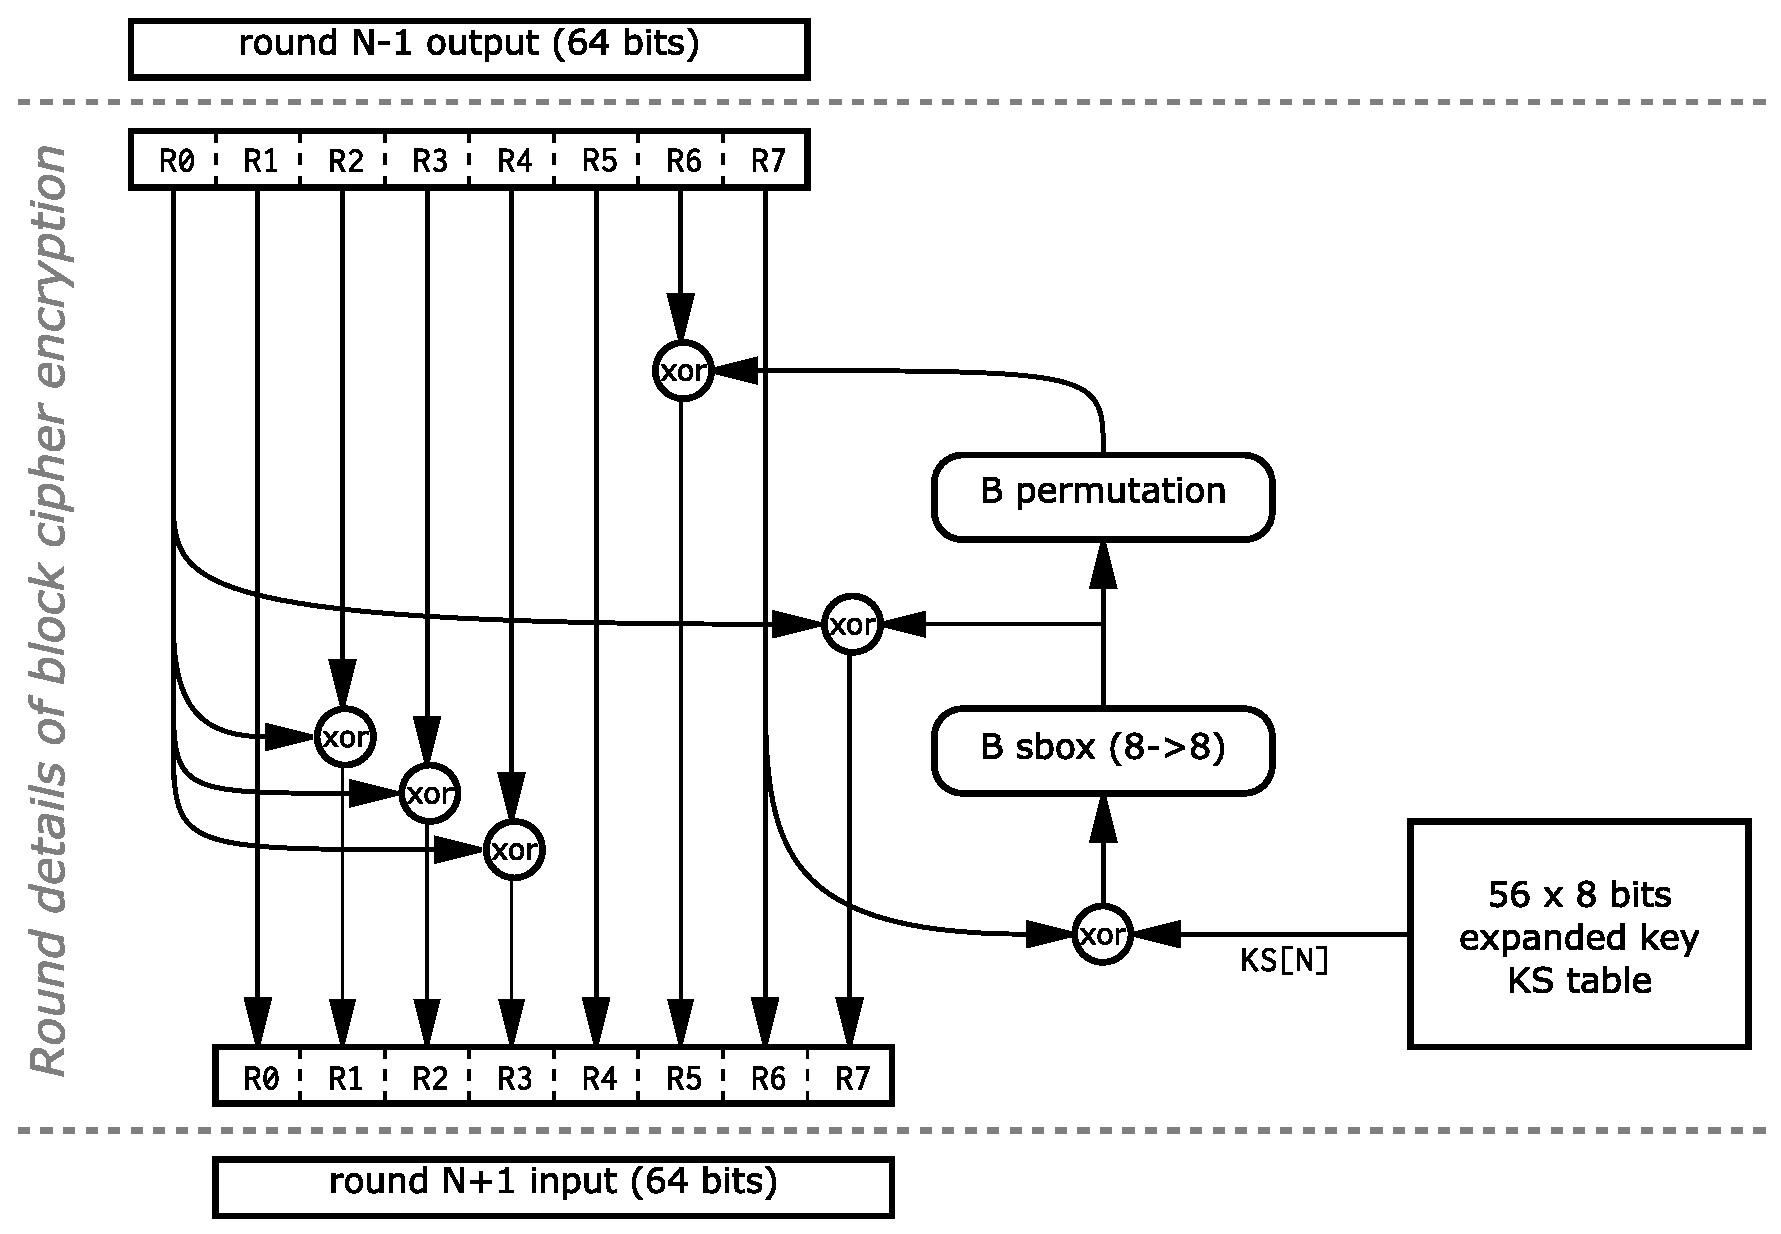
\includegraphics[width=\columnwidth/10*7]{Dvbcsa_block_encrypt}
  \caption{Подробный разбор алгоритма блочного скремблирования DVB }\label{Dvbcsa_block}
\end{figure}

\subparagraph{Потоковые шифры}%
Потоковые шифры представляют собой разновидность гаммирования и преобразуют
открытый текст в шифрованный последовательно по 1 биту. Генератор ключевой
последовательности выдаёт последовательность бит $k_1,k_2, \ldots,k_i, \ldots
$ Эта ключевая последовательность складывается по модулю 2 с
последовательностью бит исходного текста $p_1,p_2, \ldots,p_i, \ldots $ для
получения шифрованного текста:

\begin{equation}\label{potocShifr}
c_i=p_i \oplus k_i;
\end{equation}
На приемной стороне шифрованный текст складывается по мо­дулю 2 с идентичной
ключевой последовательностью для получения исходного текста:

\begin{equation}\label{potocShifr}
c_i \oplus k_i =p_i \oplus k_i \oplus k_i=p_i;
\end{equation}

%%% ANALYSIS OF THE DVB COMMON SCRAMBLING ALGORITHM, 2004
\begin{figure}[!ht]
  \centering
  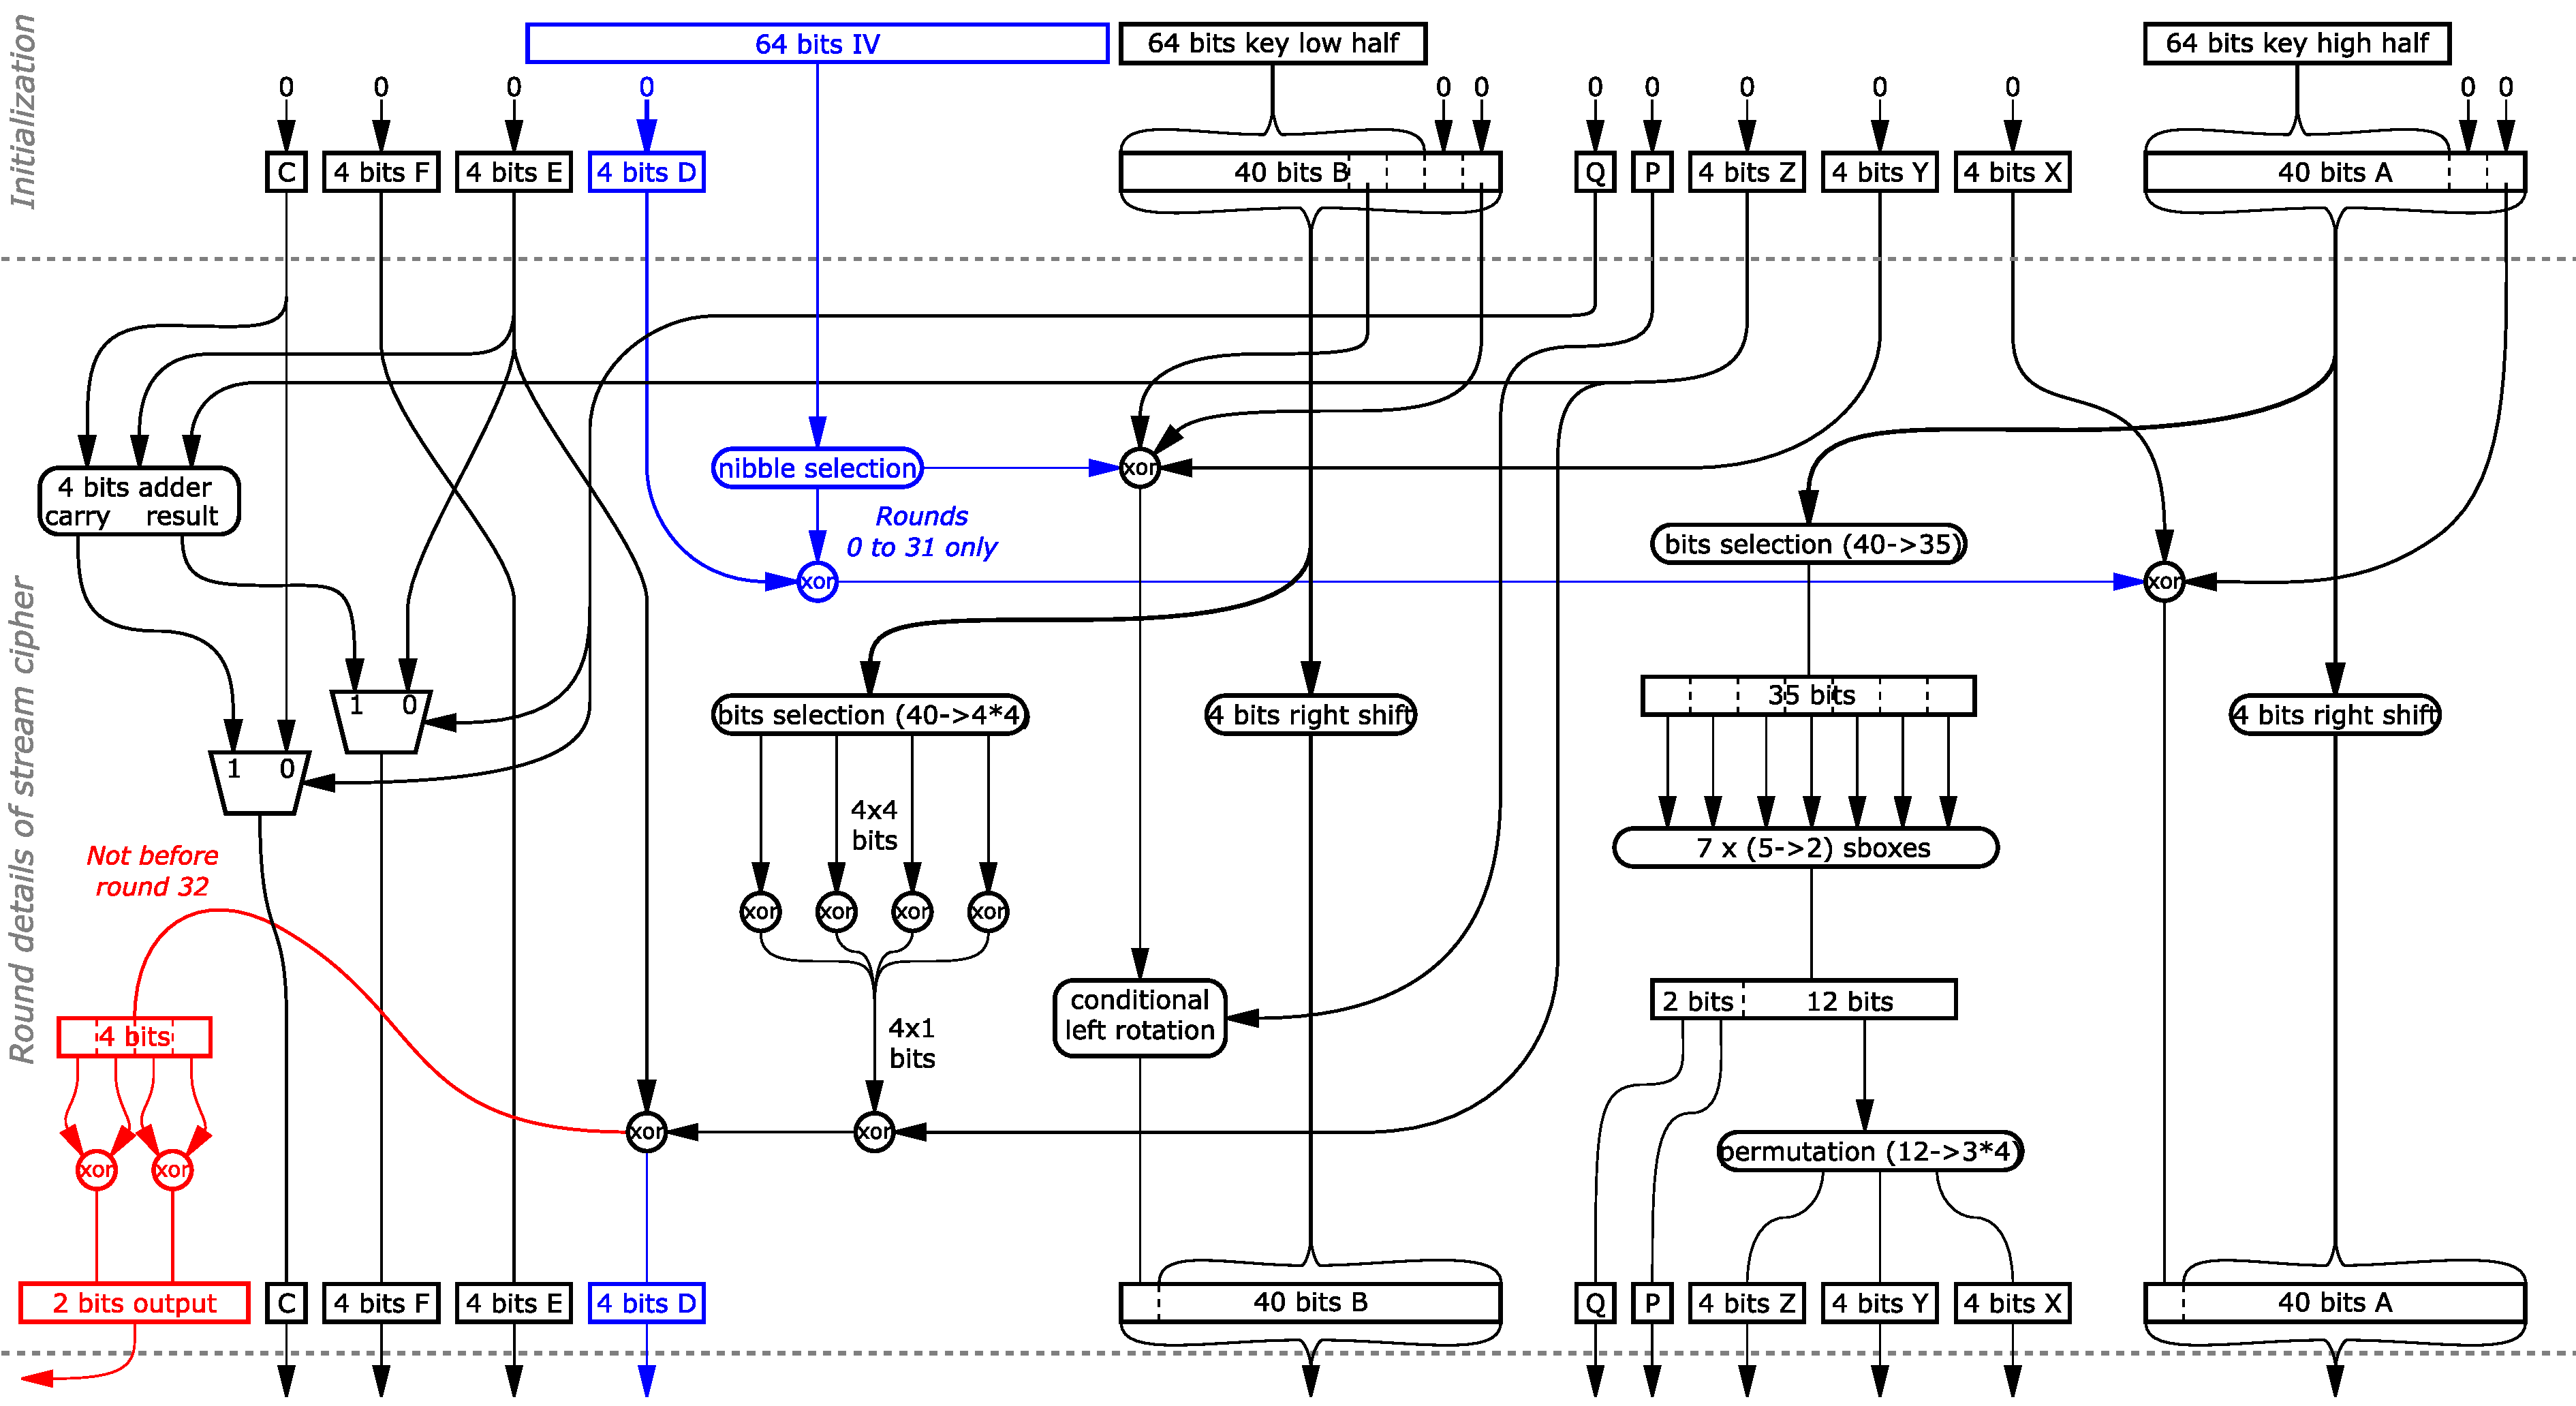
\includegraphics[width=\columnwidth]{Dvbcsa-stream}
  \caption{Подробный разбор алгоритма потокового скремблирования DVB }\label{Dvbcsa_stream}
\end{figure}
%%% https://studfiles.net/preview/1464213/
Стойкость системы целиком зависит от внутренней структуры генератора ключевой
последовательности. Если генератор выдаёт последовательность с небольшим
периодом, то стойкость системы будет невелика. Напротив, если генератор будет
выдавать бесконечную последовательность истинно случайных бит, то мы получим
«ленту однократного использования» с идеальной стойкостью.

Реальная стойкость потоковых шифров лежит где-то посредине между стойкостью
простой моноалфавитной подстановки и «ленты однократного использования».
Генератор ключевой последовательности выдаёт поток битов, который выглядит
случайным, но в действительности является детерминированным и может быть в
точности воспроизведен на приемной стороне. Чем больше генерируемый поток
похож на случайный, тем больше усилий потребуется от криптоаналитика для
взлома шифра.

\subparagraph{Криптографические протоколы} %
В современной криптографии большое внимание уделяется не только созданию и
исследованию шифров, но и разработке криптографических протоколов.

\textbf{Протокол} --- это последовательность шагов, которые предпринимают две
или большее количество сторон для совместного решения задачи. Все шаги
следуют в порядке строгой очередности, и ни один из них не может быть сделан
прежде, чем закончится предыдущий. Кроме того, любой протокол подразумевает
участие, по крайней мере, двух сторон.

%https://www.intuit.ru/studies/courses/691/547/lecture/12371?page=4
\textbf{Криптографический протокол} --- это такая процедура взаимодействия
двух или более абонентов с использованием криптографических средств, в
результате которой \emph{абоненты} достигают своей цели, а их
\emph{противники} -- не достигают. В основе протокола лежит набор правил,
регламентирующих использование криптографических преобразований и алгоритмов
в информационных процессах. Каждый криптографический протокол предназначен
для решения определённой задачи.

Рассмотрим простейший протокол для обмена конфиденциальными сообщениями между
двумя сторонами, которые будем называть \texttt{абонент №1} и \texttt{абонент
№2}. Пусть \texttt{абонент №1} желает передать зашифрованное сообщение
\texttt{абоненту №2}. В этом случае их последовательность действий должна
быть следующей.
\begin{enumerate}
  \item Абоненты выбирают систему шифрования \emph{(например, шифр
      Цезаря)}.
  \item Абоненты договариваются о ключе шифрования.
  \item \texttt{Абонент №1} шифрует исходное сообщение с помощью ключа
      выбранным
      методом
      и получает зашифрованное сообщение.
  \item Зашифрованное сообщение пересылается \texttt{абоненту №2}.
  \item \texttt{Абонент №2} расшифровывает зашифрованное сообщение с помощью
      ключа и
      получает открытое сообщение.
\end{enumerate}
Этот протокол достаточно прост, однако он может действительно использоваться
на практике. Криптографические протоколы могут быть простыми и сложными в
зависимости от назначения.

\paragraph{Сферы применения криптографии.}%
В настоящее время криптография прочно вошла в нашу жизнь. Перечислим лишь
некоторые сферы применения криптографии в современном информатизированном
обществе:
\begin{itemize}
  \item шифрование данных при передаче по открытым каналам связи (например,
      при совершении покупки в Интернете сведения о сделке);
  \item обслуживание банковских пластиковых карт;
  \item хранение и обработка паролей пользователей в сети;
  \item сдача бухгалтерских и иных отчётов через удалённые каналы связи;
  \item банковское обслуживание предприятий через локальную или глобальную сеть;
  \item безопасное от несанкционированного доступа хранение данных на
      жёстком диске компьютера.
\end{itemize}

\noindent Средства обеспечения информационной безопасности можно разбить на
четыре группы:
\begin{itemize}
  \item организационные средства (действия общего характера,
      предпринимаемые руководством организации, и конкретные меры
      безопасности, имеющие дело с людьми);
  \item законодательные средства (стандарты, законы, нормативные акты и
      т.д.);
  \item программно-аппаратные средства (системы идентификации и
      аутентификации; системы шифрования дисковых данных;
  \item системы аутентификации электронных данных и т.д.);
  \item криптографические средства (электронная цифровая подпись,
      шифрования, аутентификация и др.).
\end{itemize}

\paragraph{Оценка надёжности шифров}
Методы оценки качества криптоалгоритмов, используемые на практике:

\begin{enumerate}
  \item всевозможные попытки их вскрытия;
  \item анализ сложности алгоритма дешифрования;
  \item оценка статистической безопасности шифра.
\end{enumerate}

\noindent \textbf{В первом случае} многое зависит от квалификации, опыта,
интуиции криптоаналитика и от правильной оценки возможностей противника.
Обычно считается, что противник знает шифр, имеет возможность его изучения,
знает некоторые характеристики открытых защищаемых данных, например тематику
сообщений, их стиль, стандарты, форматы и т. п. Рассмотрим следующие примеры
возможностей противника:
\begin{Notes}
  \item противник может перехватывать все зашифрованные сообщения, но не
      имеет соответствующих им открытых текстов;
  \item противник может перехватывать все зашифрованные сообщения и
      добывать соответствующие им открытые тексты;
  \item противник имеет доступ к шифру (но не ключам!) и поэтому может
      зашифровывать и расшифровывать любую информацию.
\end{Notes}

\noindent \textbf{Во втором случае} оценку стойкости шифра заменяют оценкой
минимальной сложности алгоритма его вскрытия. Однако получение строго
доказуемых оценок нижней границы сложности алгоритмов рассматриваемого типа
не представляется возможным. Иными словами, всегда возможна ситуация, когда
алгоритм вскрытия шифра, сложность которого анализируется, оказывается вовсе
не самым эффективным.

Сложность вычислительных алгоритмов можно оценивать числом выполняемых
элементарных операций, при этом, естественно, необходимо учитывать их
стоимость и затраты на их выполнение. В общем случае это число должно иметь
строгую нижнюю оценку и выходить за пределы возможностей современных
компьютерных систем. Качественный шифр невозможно раскрыть способом более
эффективным, чем полный перебор по всему ключевому пространству, при этом
криптограф должен рассчитывать только на то, что у противника не хватит
времени и ресурсов, чтобы это сделать.

Алгоритм полного перебора по всему ключевому пространству это пример так
называемого экспоненциального алгоритма. Если сложность алгоритма выражается
неким многочленом (полиномом) от п, где п - число элементарных операций,
такой алгоритм носит название полиномиального.

\noindent \textbf{В третьем случае} считается, что надежная криптосистема с
точки зрения противника
 является <<чёрным ящиком>>, входная и выходная информационные последовательности
которого взаимно независимы, при этом выходная зашифрованная последовательность
является псевдослучайной. Поэтому смысл испытаний заключается в проведении статистических
 тестов, устанавливающих зависимость изменений в зашифрованном тексте от изменений
 символов или битов в исходном тексте или ключе, а также анализирующих, насколько
 выходная зашифрованная последовательность по своим статистическим свойствам
приближается к истинно случайной последовательности. Случайность текста шифровки
 можно приближённо оценивать степенью её сжатия при использовании алгоритма Лемпела-Зива,
 применяемого в архиваторах IBM PC. Если степень сжатия больше $10\%$, то можно
 считать криптосистему несостоятельной.

\section{Задания}\label{sect1_b}
% https://studfiles.net/preview/2905518/page:5/
%  Лаб 10
Выполнение первой работы предусматривает две части. Нужно реализовать
шифровку ручными методами, не используя ПО. Вторая часть предусматривает
использование специализированного ПО. После выполнения обеих частей требуется
сравнить результате, записать выводы.

Выполнение действий должно сопровождаться соответствующими заметками в
отчёте.

\noindent Уровень 1.%
\begin{enumerate}
    \item Зашифровать 5-ю различными методами свои ФИО.
    \item Приложить ключи к отчёту.
    \item Составить инструкцию для расшифровки.
    \item Выбрать данные соответствующие варианту из \todo{табл.}
    \item Используя данные по варианту расшифровать криптотекст.
    \item Записать результаты в отчёт.
  \end{enumerate}

\noindent Уровень 2.%*

\begin{enumerate}
  \item Используя ключ из \todo{табл.} определить шифр.
  \item Написать алгоритм шифровки-дешифровки заданным способом. Алгоритм
      должен быть представлен в виде подробной блок-схемы.
\end{enumerate}
\section{Пример выполнения работы}\label{sect1_c}
%

\section{Вопросы для контроля}\label{sect1_e}
%
\begin{enumerate}
    \item Криптография и её роль в обществе.
    \item Объяснить цель и задачи криптографии.
    \item Пояснить какие бывают криптографические методы.
    \item Виды криптографии и их классификация.
    \item Отличие симметричных и асимметричный шифров.
    \item Пояснить что такое исходный текст, шифр, ключ.
    \item Принцип подбора ключа в симметричных криптосистемах.
    \item Принцип работы симметричных шифров. Приведите примеры.
    \item Принцип работы асимметричных шифров. Приведите примеры.
    \item Преимущества и недостатки симметричный систем.
    \item Шифры одиночной перестановки и перестановки по ключевому слову. Шифр
        Гронфельда.
    \item Шифры двойной перестановки. Шифрование с помощью магического
        квадрата.
    \item Шифр многоалфавитной замены и алгоритм его реализации.
    \item Пояснить алгоритм шифрации двойным квадратом. Шифр Enigma.
\end{enumerate}

\chapter{Работа с PKI} \label{chapt2}%
\textbf{Мета роботи:~}%
Изучить методы генерации простых чисел, проверку на простоту числа и
реализовать алгоритм Диффи-Хелмана.
\section{Теоретические ведомости} \label{sect2_a}
% Лабораторная 2
Асимметричные криптографические системы были разработаны в 1970-х гг.
Принципиальное отличие асимметричной криптосистемы от криптосистемы
симметричного шифрования состоит в том, что для шифрования информации и её
последующей расшифровки используются различные ключи: открытый ключ К
\begin{Notes}
\item используется для шифрования информации, вычисляется из секретного ключа
    к;
\item секретный ключ к используется для расшифровки информации,
    зашифрованной с помощью парного ему открытого ключа К.
\end{Notes}

Эти ключи различаются таким образом, что с помощью вычислений нельзя вывести
секретный ключ к из открытого ключа К. Поэтому открытый ключ К может свободно
передаваться по каналам связи.
Асимметричные системы называют также
двухключевыми криптографическими системами, или криптосистемами с открытым
ключом.

Обобщенная схема асимметричной криптосистемы шифрования с открытым ключом
показана на \todo{рис ниже}
\begin{figure}[h]
  \centering
  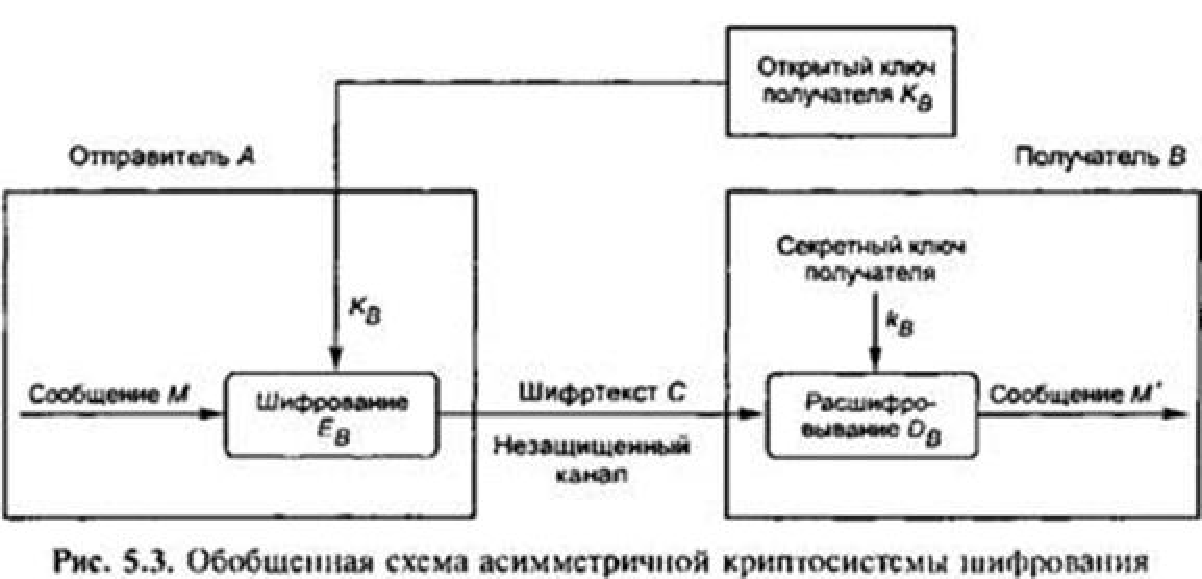
\includegraphics[width=\linewidth]{lab-2_1}
  \caption{Обобщённая схема асимметричной криптосистемы шифрования}\label{img:2_1}
\end{figure}

Для криптографического закрытия и последующего расшифровки передаваемой
информации используются открытый и секретный ключи получателя В сообщения. В
качестве ключа зашифровки должен использоваться открытый ключ получателя, а в
качестве ключа расшифровки — его секретный ключ.

Секретный и открытый ключи генерируются попарно. Секретный ключ должен
оставаться у его владельца и быть надежно защищен от НСД (аналогично ключу
шифрования в симметричных алгоритмах). Копия открытого ключа должна
находиться у каждого абонента криптографической сети, с которым обменивается
информацией владелец секретного ключа.

\paragraph{Передача ключа}
Процесс передачи зашифрованной информации в асимметричной криптосистеме
осуществляется следующим образом.

\subparagraph{Подготовительный этап}
\begin{itemize}
  \item абонент В генерирует пару ключей: секретный ключ кв и открытый ключ
      Кв;
  \item открытый ключ Кв посылается абоненту А и остальным абонентам (или
      делается доступным, например на разделяемом ресурсе).
\end{itemize}

\subparagraph{Обмен информацией между абонентами А и В}
\begin{itemize}
  \item абонент А шифрует сообщение с помощью открытого ключа Кв абонента В
      и отправляет шифротекст абоненту В;
  \item абонент В расшифровывает сообщение с помощью своего секретного
      ключа кв.
\end{itemize}
Никто другой (в том числе абонент А) не может расшифровать данное сообщение,
так как не имеет секретного ключа абонента В. Защита информации в
асимметричной криптосистеме основана на секретности ключа кв получателя
сообщения.

\subparagraph{Характерные особенности асимметричных криптосистем}
\begin{itemize}
  \item открытый ключ Кв и криптограмма С могут быть отправлены по
      незащищенным каналам, т. е. противнику известны Кв и С;
  \item  алгоритмы шифрования и расшифровывания: Ев : М → С; DB : С → М
      являются открытыми.
\end{itemize}
%
\paragraph{Методы генерации простых чисел}
%
Задача генерации простых чисел относится к классическим вычислительным
проблемам, известным с античных времен. С появлением криптографии с открытым
ключом эта проблема приобрела не только теоретическое, но и большое
практическое значение, так как большие случайные простые числа служат
параметрами (открытыми или закрытыми) многих асимметричных криптосистем.
Поскольку «формула» построения простого числа не известна (хотя её поисками
занимались многие выдающиеся математики), то все методы генерации простых
чисел действуют по следующей схеме: строится случайное нечетное число n
нужной длины и затем проверяется на простоту одним из известных тестов.

В 1976 г. Х. Уильямс привел следующую классификацию методов проверки чисел на
простоту (судя по более поздним публикациям, эта классификация не потеряла
актуальности по настоящее время):

Детерминированные методы, использующие специальные функции и/или знание
полного или частичного разложения числа n – 1 на простые множители. Эти
методы математически строго доказывают простоту или составность проверяемого
числа n. Методы Монте-Карло (вероятностные) – не требуют разложения на
простые множители, работают очень быстро, но не дают строгого доказательства
простоты (составности) числа. Методы гипотез – промежуточные между методами
Монте-Карло и математически строгими методами. Основаны на истинности
какой-либо недоказанной пока гипотезы (например, обобщённой гипотезы Римана):
в предположении, что гипотеза верна, эти методы превращаются в
детерминированные. Все детерминированные методы, которые были известны до
августа 2002 г., имеют экспоненциальную оценку сложности. В работе индийских
математиков M. Agrawal, N. Kayal, N. Saxena с замечательным названием
<<PRIMES is in P>> представлен детерминированный полиномиальный тест на
простоту; однако на данный момент вследствие своей сложности этот тест имеет
скорее теоретическое, чем практическое значение.

\paragraph{Известные алгоритмы}
%
\todo{Извесные алгоритмы сегодня}

\paragraph{Алгоритма Диффи-Хелмана}
%
\todo{История, цель и важность}

\subparagraph{Принцип работы алгоритма}

\todo{Отобразить принцип работы алгоритма}

\subparagraph{Пример реализации} блок схема(как там мороки много)

\section{Задания}\label{sect2_b}
%
Стандартный алгоритм для выполнения работы --- Алгоритм Диффи-Хелмана. Не
запрещено использовать более новые алгоритмы, соответствующие тем же
принципам.

Вариант задания указан в \todo{табл.}.

\noindent Уровень 1.

\begin{enumerate}
    \item Описать последовательность выполнения алгоритма для шифрования
        задания по варианту указаному выше.
  \item Исследовать использование алгоритма в различных сферах ИБ. Указать
      реальное применение данного алгоритма.
\end{enumerate}

\noindent Уровень 2.

\begin{enumerate}
  \item Составить программу для реализации алгоритма ДХ.
  \item Произвести поэтапный обмен между двумя клиентами.
  \item Предоставить все промежуточные данные, как на \todo{табл.}
  \item Продемонстрировать шифрованный блок и записать его в отчёт.
\end{enumerate}

\noindent Уровень 3.

\begin{enumerate}
  \item Разработать приложение клиент-клиент обмена информацией между
      несколькими людьми. Используя асинхронный алгоритм шифрования.
  \item Продемонстрировать выполнение приложения.
  \item Предоставить исходный код в дополнение отчёта.
\end{enumerate}
Приложение может быть составлено в любом варианте, например: онлайн передача,
запись в шифрованный файл, почтовый шифр и другие.
\section{Пример выполнения работы}\label{sect2_c}
%
\section{Варианты}\label{sect2_d}
%
\section{Вопросы для контроля}\label{sect2_e}
\begin{enumerate}
  \item Асимметричные системы.
  \item Привести примеры асимметричных алгоритмов.
  \item Криптосистемы. Использование асимметричный алгоритмов.
  \item Преимущества и недостатки асимметричный систем.
  \item Методы подбора ключа в асимметричных криптосистемах.
  \item Сферы использование асимметричных алгоритмов.
  \item Описать однонаправленные функции. Привести примеры.
\end{enumerate}
%

\chapter{Cisco. Топология сетей} \label{chapt3}%
\textbf{Мета роботи:~}%
Напомнить основные концепции сети, их связи, уязвимости  и основные узлы.
\section{Теоретические ведомости} \label{sect3_a}
%
\paragraph{Информационная среда}

Сеть со стороны ИБ.

Основые <<дыры>> в сети

\paragraph{Пути несанкционированного доступа}


\subparagraph{Средства защиты информации}

(всяко-разно)%
\href{https://ru.wikipedia.org/wiki/%D0%97%D0%B0%D1%89%D0%B8%D1%82%D0%B0_%D0%B8%D0%BD%D1%84%D0%BE%D1%80%D0%BC%D0%B0%D1%86%D0%B8%D0%B8_%D0%B2_%D0%BB%D0%BE%D0%BA%D0%B0%D0%BB%D1%8C%D0%BD%D1%8B%D1%85_%D1%81%D0%B5%D1%82%D1%8F%D1%85}%
{Ссылка на вики} по этой теме

 -- Маршрутизатор как способ защиты. (обязательно включить)
    - Фильтрование сети

    - экранирование сети

Защита информации в сети Интернет:

\section{Задания}\label{sect3_b}
%
\noindent Уровень 1.

\begin{enumerate}
  \item Изучить предложенную топологию в Cisco. Представлена на \todo{рис.}
  \item Изменить модель по варианту.
    \begin{enumerate}
    \item Построить реализацию заданной сети в Cisco или другом ПО.
    \item Указать недостатки заданной системы.
    \end{enumerate}
\end{enumerate}

\noindent Уровень 2.

\begin{enumerate}

  \item Настроить маршрутизатор по варианту.
    \begin{enumerate}
        \item Шаг 1.
        \item Шаг 2.
        \item Шаг 3.
        \item Шаг 4.
        \item Шаг 5.
        \item Шаг 6.
        \item Шаг 7.
        \item Шаг 8.
    \end{enumerate}
  \item Разделение подсети, \todo{протокол RIP}
\end{enumerate}
\section{Пример выполнения работы}\label{sect3_c}
%
\section{Варианты}\label{sect3_d}
%
\section{Вопросы для контроля}\label{sect3_e}
%
\begin{enumerate}
  \item Какие есть средства защиты частной сети?
  \item Что такое шлюз сетевого уровня?
  \item Преимущества и недостатки использования сетевых экранов.
  \item Что такое списки доступа? Каковы их цели и применение?
  \item Приведите пример списка доступа.
  \item Что такое маска подсети?
  \item Каков принцип маски и как происходит фильтрация
      пакетов
\end{enumerate}

\chapter{Электронно-цифровая подпись} \label{chapt4}%
\textbf{Мета роботи:~}%
Принцип работы, особенности, создание и использование ЭЦП.
\section{Теоретические ведомости} \label{sect4_a}
% https://www.youtube.com/watch?v=nrW_v8OBOno
% https://habrahabr.ru/post/194664/
% https://tools.ietf.org/html/rfc5280


Что такое ЭЦП. (электронная подпись)

\paragraph{Структура сертификата}
%http://rsdn.org/article/ASN/ASN.xml
\paragraph{Преимущества ЭЦП}

\paragraph{Недостатки ЭЦП}

\paragraph{Применение ЭЦП}
(Интернет, https)алгоритмы и т.д.

\subparagraph{Текущие требования к стойкости ЭЦП}

\paragraph{Проверка подлинности ЭЦП}
% http://nalog-nalog.ru/spravochnaya_informaciya/kak_proishodit_proverka_podlinnosti_ecp/
% http://referatwork.ru/category/tehnologii/view/475258_identifikaciya_i_proverka_podlinnosti
\section{Задания}\label{sect4_b}

Уровень 1. %

\begin{enumerate}
  \item Выбрать и отобразить реестр сертификатов на Вашем устройстве.
  \item Опишите состав сертификата.
  \item Выберите шифрованный блок данных.
  \item Опишите полный путь данного сертификата к \todo{main-центру раздачи
      разрешений}.
\end{enumerate}

Уровень 2. %

\begin{enumerate}
  \item Создайте самоподписной сертификат.
  \item Внесите его в свой реестр.
  \item Приложите данные в отчёт.
\end{enumerate}

Уровень 3.%

\begin{enumerate}
  \item Напишите алгоритм для создания подписанного сертификата.
  \item Создайте сертификат подписанный ЭЦП из прошлого задания.
  \item Приложите пример работы программы и подписанный сертификат.
\end{enumerate}

\section{Пример выполнения работы}\label{sect4_c}
%
Пример будет включать создание ЭПЦ как самостоятельно, так и используя ПО.
\section{Варианты}\label{sect4_d}
%
\section{Вопросы для контроля}\label{sect4_e}
%
\begin{enumerate}
  \item Что такое электронно-цифровая подпись?
  \item Каков принцип работы ЭЦП?
  \item Почему ЭЦП используется в большинстве систем проверки документации?
  \item Опишите этапы шифрования-дешифровки.
  \item Как подпись обеспечивает целостность данных?
  \item Случаи небезопасного использования ЭПЦ?
  \item Где на компьютере могут храниться цифровые подписи?
  \item Как проверить надёжность ЭПЦ?
\end{enumerate}

\chapter{Системы авторизации пользователя} \label{chapt5}%
\textbf{Мета роботи:~}%
Освоить основные принципы систем автоматической авторизации пользователя.
\section{Теоретические ведомости} \label{sect5_a}

% https://sites.google.com/site/infobezcom/11-mehanizmy-informacionnoj-bezopasnosti/tema-12-identifikacia-i-autentifikacia
% http://www.stikler.ru/solution/passport/
% https://habrahabr.ru/company/dataart/blog/262817/
\textit{<<Нужно заменить систему KERBEROS на другую с подобным принципом
работы>>}

\section{Задания}\label{sect5_b}
%
\section{Пример выполнения работы}\label{sect5_c}
%
\section{Варианты}\label{sect5_d}
%
\section{Вопросы для контроля}\label{sect5_e}
%

\chapter{Пакеты антивирусной защиты} \label{chapt6}%
\textbf{Мета роботи:~}%
Изучение способов защиты системы с помощью различного ПО. Научиться выбирать
ПО для защиты системы.
\section{Теоретические ведомости} \label{sect6_a}
% Из лабораторной рбаоты 4(автивирусы)

\textbf{Вредоносная программа }--- любое программное обеспечение,
предназначенное для получения несанкционированного доступа к вычислительным
ресурсам самой ЭВМ или к информации, хранимой на ЭВМ, с целью
несанкционированного использования ресурсов ЭВМ или причинения вреда
(нанесения ущерба) владельцу информации, и/или владельцу ЭВМ, и/или владельцу
сети ЭВМ, путём копирования, искажения, удаления или подмены информации.
\paragraph{История}
Сказать, где и когда появился первый вирус, невозможно, поскольку таких
данных в природе не существует. Если на «компьютере» Чарльза Бэббиджа, «отца»
первой вычислительной машины, вирусов ещё не было, к середине семидесятых
годов прошлого века они стали весьма распространенным и неприятным для
большинства явлением. Тем не менее, предпосылки к их созданию появились
практически сразу же с созданием первых ЭВМ.

Еще в 1940 году математик Джон фон Нейман написал книгу, в которой были
описаны самовоспроизводящиеся математические автоматы, то есть принципы,
которые легли в основу всех вирусов. В 1959 году американский научный журнал
«Scientific American» опубликовал статью Л. Пенроуза, рассказывавшую о
самостоятельно распространяющихся биологических структурах. Автор рассмотрел
способности подобных структур к мутациям, активации и размножению. Другой
ученый, Ф. Шталь, полученные из этой статьи знания реализовал на практике.
Работая оператором в научно-исследовательской лаборатории, он имел доступ к
мощнейшей для того времени ЭВМ – IBM 650. Эксперимент очень удивил Шталя,
превзойдя все его ожидания. Получившийся в результате «мутации»
математических алгоритмов электронный «зверек» удалил все следы своих
«родителей», присутствовавших в системе, после чего самоуничтожился.

Естественно, все вышеперечисленные труды и опыты были направлены не для того,
чтобы нынешние вирусописатели ежедневно выбрасывали в Интернет мегабайты
новой «заразы». Изначально эти исследования, относившиеся к области создания
искусственного интеллекта, представляли собой академический интерес. Однако
любое открытие, сделанное в мирных целях, может быть без особых трудностей
превращено в мощное оружие разрушения.

В 1961 году среди компьютерщиков была очень популярна игра «Darwin». Её сюжет
и смысл были просты: игрок руководил «расой», которая должна была уничтожить
своих конкурентов. Выигрывал тот, кто захватит всю отданную под игровой
процесс оперативную память. Особых действий в игре не требовалось: необходимо
было лишь размножить принадлежащих к своей расе на свободные ячейки ОЗУ или
же захватить ячейки противника. Подобный алгоритм очень похож на логику
работы деструктивных программ.

Широкое распространение компьютерных сетей стало катализатором появления на
свет первых деструктивных программ –-- \textbf{компьютерных вирусов}.

\subparagraph{70-е годы: начало}
%
Появление первого в мире компьютерного вируса было зафиксировано в начале
70-х годов прошлого столетия, когда на просторах военной компьютерной сети
APRAnet – прародительницы современного Интернета – была найдена программа
Creeper. Вирус был написан для распространенной в те времена операционной
системы Tenex, в которую он проникал, распространяясь через модемную связь.
На экран зараженных компьютеров периодически выводилась надпись: <<I’M THE
CREEPER: CATCH ME IF YOU CAN>>. Деструктивных действий Creeper не совершал,
ограничиваясь лишь этим сообщением, раздражавшим пользователей. Чуть позже
для него было написано <<противоядие>> -- программа Reaper, находившая файл с
вирусом и удалявшая его. Распространялась она, кстати, аналогичным с Creeper
способом. Можно сказать, что первый в мире антивирус был создан <<по аналогии
с вредоносной программой>>.

В 1974 году <<частым гостем>> на различных серверах была программа с милым
для животноводов названием Rabbit. <<Кролик>> ничего, кроме распространения и
размножения самого себя, не делал. Программа самовоспроизводилась с огромной
скоростью, постепенно занимая все системные ресурсы. Иногда Rabbit даже
вызывал сбой в работе серверов.

Другой пример – логическая игра Pervading Animal для операционной системы
Exec 8, смысл которой заключался в отгадывании пользователем загаданного
программой животного. Если ему это не удавалось, игра предлагала
модернизировать её, после чего появлялась возможность задавать дополнительные
наводящие вопросы.

Модифицированная версия программы странным образом начинала копироваться в
другие директории, в результате чего через некоторое время во всех папках
жёсткого диска содержалась копия Pervading Animal. Так как в то время каждый
килобайт пространства был <<на вес золота>>, подобное поведение игры мало
кого обрадовало. До сих пор не ясно, была ли это ошибка программистов либо же
задумка вирусописателей. Впрочем, проблема была быстро решена – новая версия
операционной системы Exec 8 базировалась на другом типе файловой системы, на
которой программа засорять файловое пространство больше не могла.

\subparagraph{80-е: первые эпидемии}
%
К восьмидесятым годам прошлого столетия компьютер перестал быть роскошью,
доступной лишь избранным. Владельцев ПК становится все больше, кроме того,
обмен информацией между пользователями с помощью электронных досок объявлений
(BBS – Buletin Board System) достиг международного масштаба.

В 1981 году произошла первая по-настоящему массовая вирусная эпидемия.
Пострадали широко распространенные в то время компьютеры Apple II. Вирус Elk
Clone записывался в загрузочные секторы дискет в момент обращения к ним
пользователя. Elk Clone искажал изображение на мониторе, выводил на экран
различные текстовые сообщения, заставлял мигать текст. Неискушенные
пользователи впадали от действий вируса в оцепенение, в то время как он сам
продолжал <<перемещаться>> с одного компьютера на другой.

В 1983 году американский программист Лен Эйделман впервые употребил термин
<<вирус>>, которым он обозначил саморазмножающиеся программы.

Спустя год Фред Коэн, один из самых авторитетных вирусологов, дал четкое
определение понятию <<компьютерный вирус>>: <<программа, способная
<<заражать>> другие программы при помощи их модификации с целью внедрения
своих копий>>.

В 1986 году 19-летний пакистанец Басит Фарук Алви написал вирус Brain. Также
как и Elk Clone, Brain поражал загрузочные сектора дискет. Программа не была
ориентирована на какие-либо разрушительные функции, она лишь меняла метку
всех дискет на <<(С)Brain>>. Как утверждает автор, он преследовал только одну
цель – выяснить уровень компьютерного пиратства у себя в стране. Но уже через
несколько недель после активации вируса зараженными оказались тысячи
компьютеров по всему миру, что вызвало настоящий переполох среди
пользователей и бурю обсуждений в средствах массовой информации. В Brain был
впервые использован прием, когда при чтении зараженного сектора диска вирус
подставлял вместо этого раздела незараженный.

В 1988 году была создана первая вредоносная программа, которая не просто
заражала компьютер, но и наносила ему реальный вред. Этот вирус был создан в
Лехайском университете, в котором, кстати, работал ранее упоминавшийся Фред
Коэн. Вирус Lehigh уничтожал информацию на дисках, поражая системные файлы
COMMAND.COM. Наличие квалифицированных специалистов в университете оказалось
спасением – за стены учебного заведения он так и не пробрался. Впрочем,
немалую роль в устранении угрозы эпидемии сыграл и алгоритм самого Lehigh –
во время форматирования винчестеров он самоуничтожался вместе с остальной
информацией.

В это же время начало активно развиваться программное обеспечение, защищавшее
компьютеры от вирусов. Антивирусные программы того времени представляли собой
простенькие сканеры, которые посредством контекстного поиска пытались
обнаружить вирусный код в программах. Другим распространенным <<лекарством>>
от вредоносных программ того времени были <<иммунизаторы>>. Этот тип ПО
модифицировал все программы таким образом, чтобы вирусы считали их уже
зараженными и не выполняли по отношению к ним никаких действий. После того
как количество вирусов возросло в тысячи раз, использование иммунизаторов
было уже бесполезным.

Антивирусные фирмы чаще всего состояли из двух-трех человек и свои продукты
продавали за символическую сумму либо раздавали бесплатно. Но
распространенность защитных программ была очень низка, да и непрерывное
появление новых вирусов делало их бессильными. Интернет в то время ещё не
успел <<вырваться>> из <<объятий>> учёных и военных, а обновляться без
наличия глобальной сети было практически невозможно.

В середине 80-х годов появился термин <<Virus Hoax>> – <<вирусная
мистификация>>. В конце восьмидесятых пользователи панически боялись вирусов:
мифы о программах, выводящих из строя аппаратную часть ПК, будоражили ум
каждого владельца компьютера. Virus Hoax были ничем иным, как ложными слухами
о новых компьютерных эпидемиях. Вспоминается история, когда один шутник
разослал на разные BBS сообщения о появлении нового вируса, который
распространялся через модемы, работавшие со скоростью передачи информации
2400 бит в секунду. Чтобы не заразиться вирусом, автор рекомендовал перейти
на модемы со скоростью 1200 бит/с. И что вы думаете? Масса пользователей
выбросила более быстрые модемы ради своей <<безопасности>>.

В 1988 произошла первая эпидемия, вызванная сетевым компьютерным вирусом.
Впоследствии такие вирусы стали именоваться <<червями>>. Созданная неким
Робертом Моррисом программа поражала компьютеры, работавшие под ОС UNIX. В
планы создателя не входило нанесение вреда системе, червь должен был лишь
проникнуть в сеть ARPAnet и оставаться там незамеченным. Вирус обладал
возможностью вскрытия паролей в ОС, и в списке выполнявшихся процессов детище
Морриса отображалось в виде обычного пользовательского процесса. Червь
стремительно саморазмножался и пожирал все свободные ресурсы компьютера,
вследствие чего из строя выходили целые серверы. Некоторые из них смогли
вернуться к работе лишь через пять суток, поскольку вакцины против червя не
существовало. За время своего <<хождения по миру>> вирус поразил около 6000
компьютерных систем, затронув даже компьютеры исследовательского центра NASA.
Роберт Моррис отделался 400 часами общественных работ, но вошел в историю как
автор первого разрушительного сетевого червя.
%
\subparagraph{90-е: полиморфные вирусы}
%
В начале 90-х годов прошлого столетия английская компания Sophos, в которой
работали Ян Храске, Эд Уайлдинг и Питер Лэймер, приступила к выпуску журнала
<<Virus Bulletin>>. Virus Bulletin рассказывал о компьютерных вирусах, а
также обо всех аспектах защиты от них. Авторами журнала являлись
программисты, руководители антивирусных компаний, разработчики ПО. Журнал был
некоммерческим: за всю его историю в нем не было напечатано ни одного
рекламного объявления. Из-за этого Virus Bulletin не получил широкой
распространенности. Его читателями были в основном профессионалы в сфере IT
(информационных технологий), а также сотрудники компьютерных фирм.

В 1990 году появился новый тип вредоносных программ – полиморфные вирусы.
<<Полиморфизмом>> была названа технология, при которой вирус нельзя было
обнаружить сканером, искавшим вирусы с помощью фрагментов уже известного
вредоносного кода. Полиморфизм позволяет программам генерировать код во время
исполнения, в результате чего копия вируса на каждом новом заражённом
компьютере будет отличаться от предыдущей. Первым подобным вирусом стал
Chameleon, написанный Марком Вашбёрном. После появления полиморфных программ
неотъемлемой частью антивируса стал эмулятор для дешифрации кодов, впервые
использованный Евгением Касперским.

В этом же году в Болгарии, которая тогда была центром мирового вирусописания,
появилась специализированная BBS, с которой каждый желающий мог скачать
вредоносные программы. Конференции, посвященные программированию вирусов,
появились и в UseNet.

В это же время была опубликована книга <<Маленькая Черная Книжка о
Компьютерных Вирусах>> Марка Людвига. Она стала <<Библией>> всех создателей
вирусов. Была сформирована так называемая <<VX-сцена>> – сообщество
программистов, специализирующихся на создании компьютерных вирусов.

%
\subparagraph{Конструкторы вредоносных программ}
%
В 1992 году хакер, известный под ником Dark Avenger, выпустил в свет утилиту
MtE (Mutation Engine). С её помощью любой, даже самый примитивный вирус можно
было сделать полиморфным. Этим же человеком был впервые создан вирус Peach,
наделенный способностью обходить антивирусное ПО. Peach удалял базу изменений
программы Central Point AntiVirus. Эта программа, не находив свою базу
данных, считала, что запущена впервые, и создавала её вновь. Таким образом,
вирус обходил защиту и продолжал заражать систему.

Группа программистов, известная в сети, как Nowhere Man, выпустила
конструктор вирусов VCL (Virus Creation Laboratory). Отныне любой школьник,
даже не владеющий языками программирования, мог вооружиться конструктором и
собрать вирус любого типа и разрушительной силы. С появлением VCL и так
немалый <<поток>> новых компьютерных вредителей стал просто огромным.
%
\subparagraph{Первый арестованный вирусописатель}

На протяжении 1993-94 годов свет увидели новые конструкторы вирусов: PS-MPC и
G2. Сгенерированные ими вредоносные программы стали самой распространенной
опасностью в Интернете.

В это же время состоялся настоящий <<бум>> среди производителей антивирусов –
их программы, наконец-то, стали обязательной составляющей к практически любой
ОС. На рынок безопасности решила проникнуть даже Microsoft, выпустившая
Microsoft AntiVirus (MSAV). Первоначально программа была популярна, но
впоследствии крупнейший производитель программного обеспечения в мире
прекратил разработку продукта.

Лидерство в этой области постепенно завоевала компания Symantec, частью
которой стали крупнейшие производители антивирусного программного
обеспечения: Central Point и Fifth Generation Systems.

Эпидемия нового полиморфного вируса, Pathogen, уже не была событием из ряда
вон выходящим, к подобного рода событиям все уже начали привыкать. Однако это
был первый вирус, автор которого был найден и осуждён. Безработный Кристофер
Пайл за создание вредоносных программ был приговорен к 18 месяцам тюремного
заключения.

%
\subparagraph{Атака на Microsoft}
%
В 1995 году все разосланные бета-тестерам диски с операционной системой
Windows 95 были заражены загрузочным вирусом Form. К счастью, один из них
обнаружил неладное, и на прилавки магазинов поступила нормальная,
незараженная система.

В августе того же года появился первый макровирус, написанный на языке
WordBasic, встроенном в текстовый редактор MS Word. Макровирусом Concept были
заражены сотни тысяч компьютеров по всему земному шару, вследствие чего он
еще долго лидировал в статистических исследованиях компьютерных журналов.

В 1996 году первую эпидемию пережили пользователи Windows 95 – их компьютеры
были поражены загрузочным вирусом Boza. В июле того же года создатели
макровирусов переключились с Word на редактор электронных таблиц MS Excel,
выпустив для него вирус Laroux.

Не заставили себя ждать и резидентные вирусы, использующие сервисы <<нулевого
кольца>> ОС. Win95.Punch загружался в систему как VxD-драйвер, перехватывал
обращения к файлам и заражал их.

%
\subparagraph{Антивирусные склоки}
%
К 1997 году операционная система Linux, ранее считавшаяся оплотом <<чистоты и
стабильности>>, больше не являлась платформой, свободной от вирусов.
Linux.Bliss, распространявшийся посредством конференций UseNet, заражал
исполняемые файлы этой ОС.

В этом же году было отмечено появление двух новых типов червей,
распространявшихся через IRC и FTP. Особо большим их количеством мог
<<похвастаться>> IRC, во многом из-за своей популярности, а также
многочисленных <<дыр>> mIRC – основного клиента подобных сетей.

Под конец ХХ века в погоне за лидерством стали нередки скандалы среди
производителей антивирусов. Так, представители компании McAfee объявили о
том, что ее программисты обнаружили ошибку в антивирусе фирмы Dr.Solomon’s.
Суть заявления сводилась к тому, что Dr.Solomon’s мог находить новые и
технически совершенные вирусы только в специальном <<усиленном>> режиме, в
который переключался лишь после нахождения обычных, примитивных червей. В
результате антивирус показывал хорошие скоростные результаты при сканировании
незараженных дисков, и отличные показатели обнаружения при работе с
зараженными файлами. В ответ Dr.Solomon`s подала иск в суд на McAfee,
причиной которого стала её <<некорректно построенная рекламная компания>>. В
итоге вся <<заварушка>> завершилась покупкой McAfee контрольного пакета акций
Dr.Solomon`s.

Спустя некоторое время публичное заявление сделали тайваньские разработчики
из фирмы Trend Micro, обвинившие McAfee и Symantec в якобы <<нарушении их
патента на сканирование данных>>. Миру были сразу представлены доказательства
о <<безгрешности>> компаний, однако Trend Micro добилась своего, получив
отменную бесплатную рекламу в средствах массовой информации.
%
\subparagraph{Наиболее разрушительные вирусы}
%
Продолжать подробную историю компьютерных вирусов вплоть до наших дней не
имеет смысла, поскольку ежегодно появляются сотни и тысячи новых вредоносных
программ. Я ограничусь лишь кратким рассказом о самых известных вирусах,
появившихся после 1997 года:

\textbf{CIH} (1998) -- ущерб, нанесенный вирусом, составил порядка 80
миллионов долларов. Вирус был написан программистом из Тайваня, и стал одним
из самых разрушительных в истории. <<Чих>> заражал исполняемые файлы и
активировался каждый год 26 апреля – в день годовщины аварии на Чернобыльской
АЭС. CIH перезаписывал FlashBIOS, после чего материнские платы становились
непригодными к использованию. Первый и последний вирус, который наносил вред
аппаратной части ПК.

\textbf{Melissa} (1999) -- 26 марта 1999 года этот макровирус, распространявшийся по электронной почте, заразил около 20% офисных компьютеров по всему миру. Крупнейшие корпорации, такие как Intel, были вынуждены прекратить работу внутри своих локальных сетей. Ущерб – от 300 до 500 миллионов долларов.

\textbf{ILOVEYOU} (2000) -- скрипт, написанный на макроязыке Visual Basic.
Так же как и Melissa, распространялся по электронной почте с темой письма <<I
love you>>. Вирус рассылал свои копии по всем данным адресной книги почтового
клиента. Все логины и пароли, найденные червем на компьютере, отсылались
автору программы. Последний, кстати, и не пытался скрываться: он является
жителем Филиппин, где наказаний за компьютерные преступления не
предусмотрено.

\textbf{Code Red} (2001) -- сетевой червь, использующий ошибку в сетевом
сервисе Microsoft IIS. В заданный день зараженные компьютеры должны были
начать DDOS-атаку по списку различных серверов, среди которых были системы
правительства США. Огромные масштабы эпидемии и как итог – убытки в 2,5
миллиарда долларов.

\textbf{Blaster} (2003) -- сетевой червь, выводивший на зараженных
компьютерах сообщение о необходимости перезагрузки. Через пару дней после его
выпуска в Интернет (11 августа) были заражены миллионы компьютеров по всему
миру.

\textbf{Sobig.F} (2003) -- сетевой червь, распространявшийся по электронной
почте. Размножавшийся с огромной скоростью вирус скачивал на заражённый
компьютер дополнительные файлы, <<сжигая>> трафик и ресурсы системы.
Интересная особенность -- 10 сентября вирус прекращал свою деятельность,
больше не представляя угрозы для пользователя. Автор Sobig.F, за информацию о
котором Microsoft предлагала 250 тыс. долларов, не найден до сих пор.

\textbf{Bagle} (2004) -- сетевой червь, распространявшийся по классическому
способу, используя файловые вложения в электронных письмах. На заражённом
компьютере устанавливалась специальная <<лазейка>>, через которую
злоумышленник получал полный доступ к системе. Вирус имеет более ста
модификаций.

\textbf{MyDoom} (2004) -- в январе 2004 года этот вирус молниеносно распространился по всему Интернету, в результате чего средняя скорость загрузки сайтов в глобальной сети уменьшилась на 50%. Червю принадлежит рекорд по скорости распространения: менее чем за сутки было заражено около двух миллионов компьютеров. Точную цифру из-за масштабов эпидемии привести невозможно. Вирус был создан неизвестным программистом в качестве эксперимента, и самостоятельно прекратил свою деятельность 12 февраля того же года.

\textbf{Sasser} (2004) -- вирус вызвал <<перерыв>> в работе французских
спутниковых каналов передачи данных, отменил рейсы некоторых авиакомпаний, не
говоря уже об обычных компьютерах, чья работа была полностью приостановлена.
Распространялся Sasser благодаря ошибке в системе безопасности Windows 2000 и
XP, запуская на зараженном компьютере сканер портов. Вирус был написан
17-летним немецким школьником. Интересен тот факт, что парень запустил вирус
в сеть в День своего совершеннолетия.
%
\paragraph{Классификация}
У компаний-разработчиков антивирусного программного обеспечения существуют
собственные классификации и номенклатуры вредоносных программ. Приведённая в
этой статье классификация основана на номенклатуре <<Лаборатории
Касперского>>.

\subparagraph{По вредоносной нагрузке}
%
\begin{Notes}
  \item Помехи в работе заражённого компьютера: начиная от открытия-закрытия поддона CD-ROM и заканчивая уничтожением данных и поломкой аппаратного обеспечения. Поломками известен, в частности, Win32.CIH.   \item Блокировка антивирусных сайтов, антивирусного ПО и административных функций ОС с целью усложнить лечение.
  \item Саботирование промышленных процессов, управляемых компьютером (этим известен червь Stuxnet).
  \item Инсталляция другого вредоносного ПО.   \item Загрузка из сети (downloader).
  \item Распаковка другой вредоносной программы, уже содержащейся внутри файла (dropper).
  \item Кража, мошенничество, вымогательство и шпионаж за пользователем. Для кражи может применяться сканирование жёсткого диска, регистрация нажатий клавиш (Keylogger) и перенаправление пользователя на поддельные сайты, в точности повторяющие исходные ресурсы.   \item Похищение данных, представляющих ценность или тайну.
  \item Кража аккаунтов различных служб (электронной почты, мессенджеров, игровых серверов…). Аккаунты применяются для рассылки спама. Также через электронную почту зачастую можно заполучить пароли от других аккаунтов, а виртуальное имущество в MMOG — продать.
  \item Кража аккаунтов платёжных систем.
  \item Блокировка компьютера, шифрование файлов пользователя с целью шантажа и вымогательстваденежных средств (см. Ransomware). В большинстве случаев после оплаты компьютер или не разблокируется, или вскоре блокируется второй раз.
  \item Использование телефонного модема для совершения дорогостоящих звонков, что влечёт за собой значительные суммы в телефонных счетах.
  \item Платное ПО, имитирующее, например, антивирус, но ничего полезного не делающее (fraudware или scareware (англ.)русск.; см. тж лжеантивирус).
  \item Прочая незаконная деятельность:
  \item Получение несанкционированного (и/или дарового) доступа к ресурсам самого компьютера или третьим ресурсам, доступным через него, в том числе прямое управление компьютером (так называемый backdoor).
  \item Организация на компьютере открытых релеев и общедоступных прокси-серверов.
  \item Заражённый компьютер (в составе ботнета) может быть использован для проведения DDoS-атак.
  \item Сбор адресов электронной почты и распространение спама, в том числе в составе ботнета.
  \item Накрутка электронных голосований, щелчков по рекламным баннерам.
  \item Генерация монет платёжной системы Bitcoin.
  \item Шуточное ПО, делающее какие-либо беспокоящие пользователя вещи.
  \item Adware — программное обеспечение, показывающее рекламу.
  \item Spyware — программное обеспечение, занимающееся массовым сбором малоценной информации — например, конфигурации компьютера, каталогов диска, активности пользователя…
  \item <<Отравленные>> документы, дестабилизирующие ПО, открывающее их (например, архив размером меньше мегабайта может содержать гигабайты данных и надолго <<завесить>> архиватор).
  \item Программы удалённого администрирования могут применяться как для того, чтобы дистанционно решать проблемы с компьютером, так и для неблаговидных целей.
  \item Руткит нужен, чтобы скрывать другое вредоносное ПО от посторонних глаз. Это возможно благодаря тесной интеграции руткита с операционной системой.
  \item Иногда вредоносное ПО для собственного <<жизнеобеспечения>> устанавливает дополнительные утилиты: IRC-клиенты, программные маршрутизаторы, открытые библиотеки перехвата клавиатуры… Такое ПО вредоносным не является, но из-за того, что за ним часто стоит истинно вредоносная программа, детектируется антивирусами. Бывает даже, что вредоносным является только скрипт из одной строчки, а остальные программы вполне легитимны.
  \item Файлы, не являющиеся истинно вредоносными, но в большинстве случаев нежелательные
\end{Notes}
%
\subparagraph{По методу размножения}
%
\begin{Notes}
  \item Эксплойт --- теоретически безобидный набор данных (например,
      графический файл или сетевой пакет), некорректно воспринимаемый
      программой, работающей с такими данными. Здесь вред наносит не сам
      файл, а неадекватное поведение ПО с ошибкой. Также эксплойтом
      называют программу для генерации подобных <<отравленных>> данных.
  \item Логическая бомба в программе срабатывает при определённом условии, и
неотделима от полезной программы-носителя.
  \item Троянская программа. По своему действию является противоположностью вирусам и
червям. Его предлагают загрузить под видом законного приложения, однако
вместо заявленной функциональности он делает то, что нужно злоумышленникам.
Трояны не самовоспроизводятся и не распространяются сами по себе.Нынешние
трояны эволюционировали до таких сложных форм, как, например, бэкдор (троян,
пытающийся взять на себя администрирование компьютера) и троян-загрузчик
(устанавливает на компьютер жертвы вредоносный код).
  \item Компьютерный вирус размножается в пределах компьютера и через сменные диски.
Размножение через сеть возможно, если пользователь сам выложит заражённый
файл в сеть. Вирусы, в свою очередь, делятся по типу заражаемых файлов
(файловые, загрузочные, макро-, автозапускающиеся); по способу прикрепления к
файлам (паразитирующие, <<спутники>> и перезаписывающие) и т. д.
  \item Сетевой червь способен самостоятельно размножаться по сети. Делятся на IRC-,
почтовые, размножающиеся с помощью эксплойтов и т. д.
  \item Загрузчик --- является небольшой частью кода, используемой для дальнейшей
загрузки и установки полной версии вредоноса. После того как загрузчик
попадает в систему путем сохранения вложения электронного письма или,
например, при просмотре зараженной картинки, он соединяется с удаленным
сервером и загружает весь вредонос.
\end{Notes}
%
\paragraph{Виды антивирусной защиты}
%
\textbf{Современные антивирусы} --- это комплексные программные пакеты, как
правило, содержащие несколько взаимосвязанных и взаимодополняющих модулей,
нацеленные на борьбу со всем спектром компьютерных угроз.

\noindent В современных антивирусах могут задействоваться следующие виды
антивирусной защиты:

\textbf{Сравнение с вирусным образцом} --- вирусной сигнатурой кода, шаблоном
поведения вредоносной программы или цифровым отпечатком в <<черном>> списке
известных угроз. Эта разновидность антивирусной защиты заключается в
исследовании подозрительной программы на наличие признаков, характерных для
вредоносного ПО. Например, реализуя данный вид защиты, антивирус ищет
\textbf{сигнатуры} -- последовательности кода, уникальные для определённого
вируса.

\textbf{Поведенческий мониторинг} --- разновидность антивирусной защиты,
основанная на проверке объектов во время осуществления чтения, записи и
других операций. Для проведения мониторинга антивирусная программа
располагается в оперативной памяти и действует как обработчик системных
событий. При старте какой-либо операции, которая может привести к заражению,
антивирусный монитор запускает проверку обрабатываемого объекта (документа,
программы и т.д.).

\textbf{Обнаружение изменений} --- вид антивирусной защиты, базирующийся на
контроле целостности программных компонентов компьютера. При заражении вирусы
модифицируют файлы, системный реестр или загрузочные сектора диска.
Антивирусная программа определяет, был ли изменен объект с помощью подсчета
кодов циклического контроля (CRC-сумм) и других методов.

\textbf{Эвристический анализ}. Данный вид антивирусной защиты основан на том,
что выполняемые вирусами действия и их последовательность отличаются от
поведения большинства программ. Поэтому анализ последовательностей команд и
системных вызовов подозрительного программного обеспечения помогает выносить
правильное решение о его вредоносности.

\textbf{Лечение} --- разновидность антивирусной защиты, состоящая в удалении
вредоносных объектов и восстановлении нормальных параметров компьютерной
системы.

\textbf{Репутационный сервис} --- новейший вид антивирусной защиты,
получивший распространение в последние годы и базирующийся на проверке
репутации программ, веб-ресурсов и почтовых систем. Такая проверка проводится
с использованием <<облачных>> серверов репутации, поддерживаемых ведущими
разработчиками антивирусного ПО, и основана на постоянно обновляемых списках
<<легитимных>>, вредоносных и подозрительных ресурсов. Преимуществом
репутационных сервисов является очень высокая скорость реакции на появление
новых угроз.

Существуют и устаревшие, теперь уже редко используемые виды антивирусной
защиты, например, иммунизация, которая заключается в том, что в памяти
компьютера размещается программа, сообщающая вирусам, избегающим повторного
заражения, о том, что система уже инфицирована.

Реализуют антивирусную защиту следующие модули:
\begin{itemize}
  \item Антивирусный сканер
  \item Антивирусный монитор, использующий многочисленные технологии защиты
  \item Поведенческий блокиратор
  \item Антивирусный ревизор или система контроля CRC
  \item Антивирусный фаг или доктор.
\end{itemize}
%
\section{Задания}\label{sect6_b}
%
Уровень 1.
\begin{enumerate}
  \item По варианту выбрать систему.
  \item Исследовать систему на стойкость, защиту.
  \item Описать основные угрозы и способы взлома выбранной системы.
  \item Анализ и выбор ПО для комплексной защиты.
\end{enumerate}
Предоставить результат в виде отчета с подробным описанием слабых сторон
системы, указать способы защиты и написать инструкцию для выбранного ПО.
\section{Пример выполнения работы}\label{sect6_c}
%
\section{Варианты}\label{sect6_d}
%
\section{Вопросы для контроля}\label{sect6_e}
%

\chapter{Пассивный анализ данных} \label{chapt8}%
\textbf{Мета роботи:~}%
Изучить способы анализа данных для дальнейшего применения. Применение пакета
данных в целях защитных и атакующих систем.
\section{Теоретические ведомости} \label{sect7_a}
% https://informationsecurityweb.wordpress.com/2016/05/27/%D0%B0%D0%BD%D0%B0%D0%BB%D0%B8%D0%B7-%D1%83%D0%B3%D1%80%D0%BE%D0%B7-%D0%B8%D0%BD%D1%84%D0%BE%D1%80%D0%BC%D0%B0%D1%86%D0%B8%D0%BE%D0%BD%D0%BD%D0%BE%D0%B9-%D0%B1%D0%B5%D0%B7%D0%BE%D0%BF%D0%B0/

Зачем нужен анализ данных в ИБ.

\paragraph{Виды анализа данных}

\paragraph{Выбор средств для пассивного анализа}

Выборка и поиск атак на ресурс используя методы пасивного анализа.




\section{Задания}\label{sect7_b}
%
\begin{enumerate}
  \item Выбрать задание по варианту из \todo{табл.}
  \item Провести пассивный анализ интернет трафика.
  \item Провести выборку на массиве данных.
  \item Запустить \todo{фишинговую угрозу}.
  \item Собрать дополнительные данные и найти вирус с помощью данного
      метода.
  \item Отобразить результаты в отчёте.
\end{enumerate}
\section{Пример выполнения работы}\label{sect7_c}
%
\section{Варианты}\label{sect7_d}
%
\section{Вопросы для контроля}\label{sect7_e}
%
\begin{enumerate}
  \item Что такое анализ данных в ИБ?
  \item Какие бывают методы анализа?
  \item Какое ПО для анализа данных вы знаете?
  \item Как работает метод пассивного анализа?
  \item Как работает метод активного анализа?
  \item Какова надёжность методов анализа данных?
  \item Какие особенности, достоинства и недостатки анализа вы знаете?
\end{enumerate}

\chapter{Архивация данных} \label{chapt8}%
\textbf{Мета роботи:~}%
Выполнить исследование алгоритмов архивации данных. Использовать алгоритм
Хаффмана и Лемпеля-Зива для архивации. Восстановить данные после
\section{Теоретические ведомости} \label{sect8_a}
% Лабораторная 9
\paragraph{Архивация данных}

\textbf{Архивация (сжатие данных)} --- есть процесс представления информации
в ином виде (перекодирования) с потенциальным уменьшением объёма, требуемого
для её хранения. Существует множество классов различных алгоритмов сжатия
данных, каждый из которых ориентирован на свою область применения.
\href{http://studopedia.ru/9_131056_simmetrichnie-kriptosistemi.html}{Источник}

Основоположником науки о сжатии информации принято считать \emph{Клода
Шеннона}. Его теорема об оптимальном кодировании показывает, к чему нужно
стремиться при кодировании информации и насколько та или иная информация при
этом сожмется. Кроме того, им были проведены опыты по эмпирической оценке
избыточности английского текста. Шенон предлагал людям угадывать следующую
букву и оценивал вероятность правильного угадывания. На основе ряда опытов он
пришел к выводу, что количество информации в английском тексте колеблется в
пределах $0,6 – 1,3$ бита на символ. Несмотря на то, что результаты
исследований Шеннона были по-настоящему востребованы лишь десятилетия спустя,
трудно переоценить их значение.

\textbf{Сжатие данных} --- это процесс, обеспечивающий уменьшение объёма
данных путём сокращения их избыточности. Сжатие данных связано с компактным
расположением порций данных стандартного размера. Сжатие данных можно
разделить на два основных типа:


\textbf{Сжатие без потерь} (полностью обратимое) --- это метод сжатия данных,
при котором ранее закодированная порция данных восстанавливается после их
распаковки полностью без внесения изменений. Для каждого типа данных, как
правило, существуют свои оптимальные алгоритмы сжатия без потерь.

\textbf{Сжатие с потерями} --- это метод сжатия данных, при котором для
обеспечения максимальной степени сжатия исходного массива данных часть
содержащихся в нём данных отбрасывается. Для текстовых, числовых и табличных
данных использование программ, реализующих подобные методы сжатия, является
неприемлемыми. В основном такие алгоритмы применяются для сжатия аудио и
видеоданных, статических изображений.

\paragraph{Алгоритмы архивации данных}

\textbf{Алгоритм сжатия данных} --- это алгоритм, который устраняет
избыточность записи данных.

\textbf{Отношение сжатия} --- одна из наиболее часто используемых величин для
обозначения эффективности метода сжатия.
\begin{equation}\label{Otnosh_Schatia}
 \text{Отношение сжатия} = \frac{\text{размер
выходного потока}}{\text{размер входного потока}}
\end{equation}
Значение 0,6 означает, что данные занимают 60\% от первоначального объема.
Значения больше 1 означают, что выходной поток больше входного (отрицательное
сжатие, или расширение).

\textbf{Коэффициент сжатия} --- величина, обратная отношению сжатия.

\begin{equation}\label{Otnosh_Schatia}
 \text{Коэффициент сжатия} = \frac{\text{размер входного потока}}{\text{размер
выходного потока}}
\end{equation}
Значения больше 1 обозначают сжатие, а значения меньше 1 расширение.

\textbf{Средняя длина кодового слова} -- это величина, которая вычисляется
как взвешенная вероятностями сумма длин всех кодовых слов.

\begin{equation}
L_{cp}=p_1 \cdot L_1 + p_2 \cdot L_2 +\ldots + p_n \cdot L_n ,
\end{equation}
где $p_n$ -- вероятности кодовых слов,
    $L_1,L_2,L_3$ -- длины кодовых слов.

\textbf{Статистические методы} --- методы сжатия, присваивающие коды
переменной длины символам входного потока, причем более короткие коды
присваиваются символам или группам символам, имеющим большую вероятность
появления во входном потоке. Лучшие статистические методы применяют
кодирование Хаффмана.

\textbf{Словарное сжатие} --- это методы сжатия, хранящие фрагменты данных в
"словаре" (некоторая структура данных). Если строка новых данных, поступающих
на вход, идентична какому-либо фрагменту, уже находящемуся в словаре, в
выходной поток помещается указатель на этот фрагмент. Лучшие словарные методы
применяют метод Зива-Лемпела.

Рассмотрим несколько известных алгоритмов сжатия данных более подробно.

\subparagraph{Алгоритм Хаффмана}

В основе алгоритма Хаффмана лежит идея кодирования битовыми группами. Сначала
проводится частотный анализ входной последовательности данных, то есть
устанавливается частота вхождения каждого символа, встречащегося в ней. После
этого, символы сортируются по уменьшению частоты вхождения.

Основная идея состоит в следующем: чем чаще встречается символ, тем меньшим
количеством бит он кодируется. Результат кодирования заносится в словарь,
необходимый для декодирования. Рассмотрим простой пример, иллюстрирующий
работу алгоритма Хаффмана.

Пусть задан текст <<beep boop beer!>>, рассмотрим таблицу с частотами всех
символов:

\begin{table} [!htbp]% Пример записи таблицы с номером, но без отображаемого наименования
  \centering
  \parbox{8cm}%
  {% чтобы лучше смотрелось, подбирается самостоятельно
    \caption{Частота символов}%
    \label{tabl:tab8x1}%
    \begin{SingleSpace}
    \begin{tabular}{lccccccc}
    \hline
    \multicolumn{1}{|l|}{\textbf{Символ}}                          & \multicolumn{1}{c|}{'b'}                       & \multicolumn{1}{c|}{'e'}                       & \multicolumn{1}{c|}{'p'}                       & \multicolumn{1}{c|}{' '}                       & \multicolumn{1}{c|}{'o'}                       & \multicolumn{1}{c|}{'r'}                       & \multicolumn{1}{c|}{'!'}                       \\ \hline
    \rowcolor[HTML]{EFEFEF}
    \multicolumn{1}{|l|}{\cellcolor[HTML]{EFEFEF}\textbf{Частота}} & \multicolumn{1}{c|}{\cellcolor[HTML]{EFEFEF}3} & \multicolumn{1}{c|}{\cellcolor[HTML]{EFEFEF}4} & \multicolumn{1}{c|}{\cellcolor[HTML]{EFEFEF}2} & \multicolumn{1}{c|}{\cellcolor[HTML]{EFEFEF}2} & \multicolumn{1}{c|}{\cellcolor[HTML]{EFEFEF}2} & \multicolumn{1}{c|}{\cellcolor[HTML]{EFEFEF}1} & \multicolumn{1}{c|}{\cellcolor[HTML]{EFEFEF}1} \\ \hline
    \\
    \multicolumn{8}{c}{По частоте использования}                                                                                                                                                                                                                                                                                                                                                                             \\ \hline
    \multicolumn{1}{|l|}{\textbf{Символ}}                          & \multicolumn{1}{c|}{'r'}                       & \multicolumn{1}{c|}{'!'}                       & \multicolumn{1}{c|}{'p'}                       & \multicolumn{1}{c|}{'o'}                       & \multicolumn{1}{c|}{' '}                       & \multicolumn{1}{c|}{'b'}                       & \multicolumn{1}{c|}{'e'}                       \\ \hline
    \end{tabular}
    \end{SingleSpace}
    }
\end{table}

После этого создадим элементы бинарного дерева для каждого символа и
представим их как очередь с приоритетом, в качестве которого будем
использовать частоту.

Возьмём первые два элемента из очереди и создадим третий, который будет их
родителем. Этот новый элемент поместим в очередь с приоритетом, равным сумме
приоритетов двух его потомков. Иначе говоря, равным сумме их частот.

%2
\begin{figure}[!htbp]
  \centering
  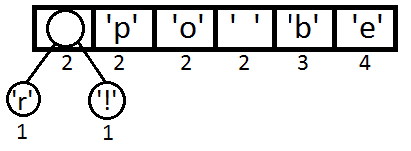
\includegraphics[width=\linewidth/3]{img8x2}
  \caption{2}\label{img:8x2}
\end{figure}
Далее будем повторять шаги, аналогичные предыдущему:

%3-6
\begin{figure}[!htbp]
  \centering
  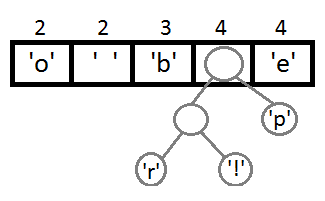
\includegraphics[width=\linewidth/3]{img8x3}
  \label{img:8x3}

  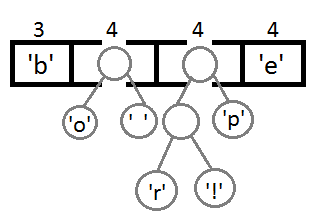
\includegraphics[width=\linewidth/3]{img8x4}
  \label{img:8x4}

  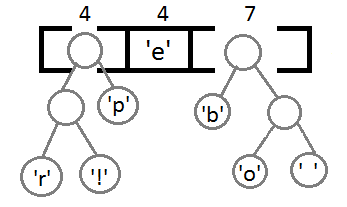
\includegraphics[width=\linewidth/3]{img8x5}
  \label{img:8x5}

  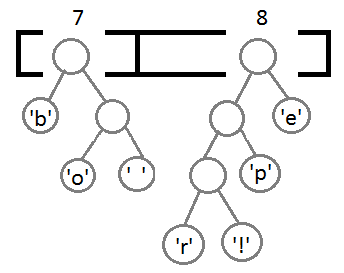
\includegraphics[width=\linewidth/3]{img8x6}
  \caption{Построение дерева}\label{img:8x6}
\end{figure}

Теперь, после объединения последних двух элементов с помощью их нового
родителя, мы получим итоговое бинарное дерево:
%7
\begin{figure}[!htbp]
  \centering
  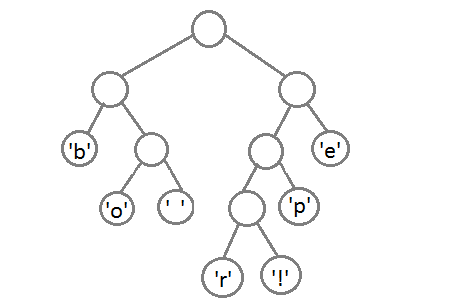
\includegraphics[scale=0.6]{img8x7}
  \caption{7}\label{img:8x7}
\end{figure}
Осталось присвоить каждому символу его код. Для этого запустим обход в
глубину и каждый раз, рассматривая правое поддерево, будем записывать в код
1, а рассматривая левое поддерево — 0.

\begin{figure}[!htbp]
  \centering
  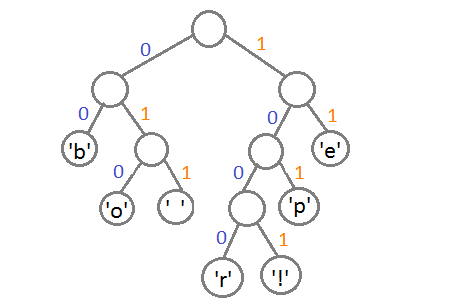
\includegraphics[scale=0.6]{img8x8}
  \caption{8}\label{img:8x8}
\end{figure}
%8

В результате соответствие символов кодовым значениям получится следующим:
\begin{table} [!htbp]% Пример записи таблицы с номером, но без отображаемого наименования
  \centering
  \parbox{12cm}%
  {% чтобы лучше смотрелось, подбирается самостоятельно
    \caption{Кодовые значения символов}%
    \label{tabl:tab8x2}%
    \begin{SingleSpace}
    \begin{tabular}{|l|c|c|c|c|c|c|c|}
    \hline
    \textbf{Сивол}            & ‘b’ & ‘e’ & ‘p’ & ‘ ‘ & ‘o’ & ‘r’  & ‘!’  \\ \hline
    \rowcolor[HTML]{EFEFEF}
    \textbf{Кодовое значение} & 00  & 11  & 101 & 011 & 010 & 1000 & 1001 \\ \hline
    \end{tabular}
    \end{SingleSpace}
    }
\end{table}

Декодирование битов происходит следующим образом: нужно обходить дерево,
отбрасывая левое поддерево, если встретилась единица и правое, если
встретился 0. Продолжать обход нужно до тех пор, пока не встретим лист, т.е.
искомое значение закодированного символа. Например, закодированной строке
<<101 11 101 11>> и нашему дереву декодирования соответствует строка <<pepe>>

\noindent \textbf{Входная строка: }<<beep boop beer!>>

\noindent \textbf{Входная строка в двоичном виде:} 0110 0010 0110 0101 0110
0101 0111 0000 0010 0000 0110 0010 0110 1111 0110 1111 0111 0000 0010 0000
0110 0010 0110 0101 0110 0101 0111 0010 0010 0001

\noindent \textbf{Закодированная строка:} 0011 1110 1011 0001 0010 1010 1100
1111 1000 1001

Разница между ASCII-кодировкой строки и её же видом в коде Хаффмана очевидна.

Алгоритм Хаффмана универсальный, его можно применять для сжатия данных любых
типов, но он малоэффективен для файлов маленьких размеров (за счет
необходимости сохранения словаря). В настоящее время данный метод практически
не применяется в чистом виде, обычно используется как один из этапов сжатия в
более сложных схемах. Это единственный алгоритм, который не увеличивает
размер исходных данных в худшем случае (если не считать необходимости хранить
таблицу перекодировки вместе с файлом).

\subparagraph{Алгоритм Лемпеля-Зива}

Процесс сжатия выглядит следующим образом. Последовательно считываются
символы входного потока и происходит проверка, существует ли в созданной
таблице строк такая строка. Если такая строка существует, считывается
следующий символ, а если строка не существует, в поток заносится код для
предыдущей найденной строки, строка заносится в таблицу, а поиск начинается
снова. Например, если сжимают байтовые данные (текст), то строк в таблице
окажется 256 (от <<0>> до <<255>>). Если используется 10-битный код, то под
коды для строк остаются значения в диапазоне от 256 до 1023. Новые строки
формируют таблицу последовательно, т. е. можно считать индекс строки ее
кодом. Алгоритму декодирования на входе требуется только закодированный
текст, поскольку он может воссоздать соответствующую таблицу преобразования
непосредственно по закодированному тексту. Алгоритм генерирует однозначно
декодируемый код за счет того, что каждый раз, когда генерируется новый код,
новая строка добавляется в таблицу строк. LZW постоянно проверяет, является
ли строка уже известной, и, если так, выводит существующий код без генерации
нового. Таким образом, каждая строка будет храниться в единственном
экземпляре и иметь свой уникальный номер. Следовательно, при дешифровании при
получении нового кода генерируется новая строка, а при получении уже
известного, строка ивлекается из словаря.
\href{https://habrahabr.ru/post/132683/}{[ссылка]}

\noindent\textbf{Кодирование}

Пусть мы сжимаем последовательность <<abacabadabacabae>>.
\begin{enumerate}
\item Тогда, согласно изложенному выше алгоритму, мы добавим к изначально
    пустой строке <<a>> и проверим, есть ли строка <<a>> в таблице. Поскольку мы
    при инициализации занесли в таблицу все строки из одного символа, то
    строка <<a>> есть в таблице.
\item Далее мы читаем следующий символ «b>> из входного потока и проверяем,
    есть ли строка <<ab>> в таблице. Такой строки в таблице пока нет.
\item Добавляем в таблицу <5> <<ab>>. В поток: <0>;
\item <<ba>> — нет. В таблицу: <6> <<ba>>. В поток: <1>;
\item <<ac>> — нет. В таблицу: <7> <<ac>>. В поток: <0>;
\item <<ca>> — нет. В таблицу: <8> <<ca>>. В поток: <2>;
\item <<ab>> — есть в таблице; <<aba>> — нет. В таблицу: <9> <<aba>>. В
    поток: <5>;
\item <<ad>> — нет. В таблицу: <10> <<ad>>. В поток: <0>;
\item <<da>> — нет. В таблицу: <11> <<da>>. В поток: <3>;
\item <<aba>> — есть в таблице; <<abac>> — нет. В таблицу: <12> <<abac>>. В
    поток: <9>;
\item <<ca>> — есть в таблице; <<cab>> — нет. В таблицу: <13> <<cab>>. В
    поток: <8>;
\item <<ba>> — есть в таблице; <<bae>> — нет. В таблицу: <14> <<bae>>. В
    поток: <6>;
\item И, наконец последняя строка <<e>>, за ней идет конец сообщения,
    поэтому мы просто выводим в поток <4>.
\end{enumerate}
\begin{figure}[!htbp]
  \centering
  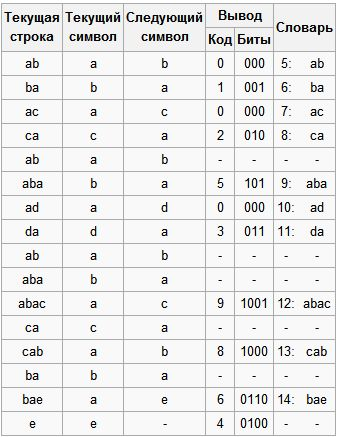
\includegraphics[scale=0.8]{img8x9}
  \caption{9}\label{img:8x9}
\end{figure}
Мы получаем закодированное сообщение <<0 1 0 2 5 0 3 9 8 6 4>>, что на
11-бит короче.\\
\vspace{1cm}
\\
\noindent\textbf{Декодирование}

Особенность LZW заключается в том, что для декомпрессии нам не надо сохранять
таблицу строк в файл для распаковки. Алгоритм построен таким образом, что мы
в состоянии восстановить таблицу строк, пользуясь только потоком кодов.
Теперь представим, что мы получили закодированное сообщение, приведённое
выше, и нам нужно его декодировать. Прежде всего, нам нужно знать начальный
словарь, а последующие записи словаря мы можем реконструировать уже на ходу,
поскольку они являются просто конкатенацией предыдущих записей.
\begin{figure}[!htbp]
  \centering
  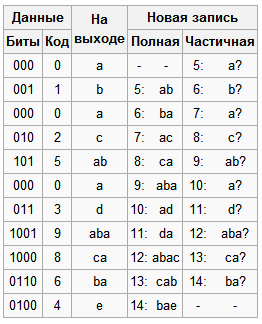
\includegraphics[scale=0.9]{img8x10}
  \caption{10}\label{img:8x10}
\end{figure}

\noindent\textbf{Достоинства и недостатки}
\begin{description}
  \item[+] Не требует вычисления вероятностей встречаемости символов или
      кодов.
  \item[+] Для декомпрессии не надо сохранять таблицу строк в файл для
      распаковки. Алгоритм построен таким образом, что мы в состоянии
      восстановить таблицу строк, пользуясь только потоком кодов.
  \item[+] Данный тип компрессии не вносит искажений в исходный графический
      файл, и подходит для сжатия растровых данных любого типа.
  \item[-]Алгоритм не проводит анализ входных данных поэтому не оптимален.
\end{description}

\section{Задания}\label{sect8_b}
%https://studfiles.net/preview/5855938/
\begin{enumerate}
  \item Взять данные соответственно варианту из \todo{табл.}
  \item Удалить лишнюю информацию методом Хаффмана.
  \item Провести операцию методом Лемпеля-Зива.
  \item Сравнить результаты проведённых операций.
  \item Описать актуальность архивации.
  \item Сделать выводы по применению методов сжатия в различных
      криптосистемах.
\end{enumerate}
\section{Пример выполнения работы}\label{sect8_c}
%
\section{Варианты}\label{sect8_d}
%
\section{Вопросы для контроля}\label{sect8_e}
%
\begin{enumerate}
  \item Что такое архивация данных?
  \item Цель архивации?
  \item Какие Вы знаете методы архивации?
  \item Опишите принцип дерева Хаффмана.
  \item Опишите алгоритм LZ77 или его аналог.
  \item Сферы применения заданных алгоритмов.
  \item Как выбрать алгоритм, если данные заранее известны?
\end{enumerate}

%\chapter{~} \label{chapt9}%
\textbf{Мета роботи:}%
%
\section{Теоретические ведомости} \label{sect9_a}
%
\section{Задания}\label{sect9_b}
%
\section{Пример выполнения работы}\label{sect9_c}
%
\section{Варианты}\label{sect9_d}
%
\section{Вопросы для контроля}\label{sect9_e}
%

             % Глава 1
  \chapter*{Рекомендації}						% Заголовок
\addcontentsline{toc}{chapter}{Заключение}	% Добавляем его в оглавление

%% Согласно ГОСТ Р 7.0.11-2011:
%% 5.3.3 В заключении диссертации излагают итоги выполненного исследования, рекомендации, перспективы дальнейшей разработки темы.
%% 9.2.3 В заключении автореферата диссертации излагают итоги данного исследования, рекомендации и перспективы дальнейшей разработки темы.
%% Поэтому имеет смысл сделать эту часть общей и загрузить из одного файла в автореферат и в диссертацию:
  % Заключение
  \clearpage                                  % В том числе гарантирует, что список литературы в оглавлении будет с правильным номером страницы
%\hypersetup{ urlcolor=black }               % Ссылки делаем чёрными
%\providecommand*{\BibDash}{}                % В стилях ugost2008 отключаем использование тире как разделителя
\urlstyle{rm}                               % ссылки URL обычным шрифтом
\ifdefmacro{\microtypesetup}{\microtypesetup{protrusion=false}}{} % не рекомендуется применять пакет микротипографики к автоматически генерируемому списку литературы
\printbibliography                         % Подключаем Bib-базы
\ifdefmacro{\microtypesetup}{\microtypesetup{protrusion=true}}{}
\urlstyle{tt}                               % возвращаем установки шрифта ссылок URL
%\hypersetup{ urlcolor={urlcolor} }          % Восстанавливаем цвет ссылок
      % Список литературы
  %\clearpage
\ifdefmacro{\microtypesetup}{\microtypesetup{protrusion=false}}{} % не рекомендуется применять пакет микротипографики к автоматически генерируемым спискам
\listoffigures  % Список изображений

%%% Список таблиц %%%
% (ГОСТ Р 7.0.11-2011, 5.3.10)
\clearpage
\listoftables   % Список таблиц
\ifdefmacro{\microtypesetup}{\microtypesetup{protrusion=true}}{}
\newpage
           % Списки таблиц и изображений (иллюстративный материал)
  \appendix
%%% Оформление заголовков приложений ближе к ГОСТ:
\setlength{\midchapskip}{20pt}
\renewcommand*{\afterchapternum}{\par\nobreak\vskip \midchapskip}
\renewcommand\thechapter{\Asbuk{chapter}} % Чтобы приложения русскими буквами нумеровались
\settocdepth{chapter}
   % Предварительные настройки для правильного подключения Приложений
%
\chapter{ДополнениеПервое} \label{AppendixA}%

\section{Очередной подраздел приложения} \label{AppendixA:1}%
%
\section{И ещё один подраздел приложения} \label{AppendixA:2}%
%
    % Приложения
\end{document}
